\documentclass[11pt]{article}

    \usepackage[breakable]{tcolorbox}
    \usepackage{parskip} % Stop auto-indenting (to mimic markdown behaviour)
    
    \usepackage{float}
    

    % Basic figure setup, for now with no caption control since it's done
    % automatically by Pandoc (which extracts ![](path) syntax from Markdown).
    \usepackage{graphicx}
    % Maintain compatibility with old templates. Remove in nbconvert 6.0
    \let\Oldincludegraphics\includegraphics
    % Ensure that by default, figures have no caption (until we provide a
    % proper Figure object with a Caption API and a way to capture that
    % in the conversion process - todo).
    \usepackage{caption}
    \DeclareCaptionFormat{nocaption}{}
    \captionsetup{format=nocaption,aboveskip=0pt,belowskip=0pt}

    \usepackage{float}
    \floatplacement{figure}{H} % forces figures to be placed at the correct 
    \usepackage{xcolor} % Allow colors to be definedhttps://www.overleaf.com/project/656f71089648add9d3ede67e
    \usepackage{enumerate} % Needed for markdown enumerations to work
    \usepackage{geometry} % Used to adjust the document margins
    \usepackage{amsmath} % Equations
    \usepackage{amssymb} % Equations
    \usepackage{textcomp} % defines textquotesingle
    % Hack from http://tex.stackexchange.com/a/47451/13684:
    \AtBeginDocument{%
        \def\PYZsq{\textquotesingle}% Upright quotes in Pygmentized code
    }
    \usepackage{upquote} % Upright quotes for verbatim code
    \usepackage{eurosym} % defines \euro

    \usepackage{iftex}
    \ifPDFTeX
        \usepackage[T1]{fontenc}
        \IfFileExists{alphabeta.sty}{
              \usepackage{alphabeta}
          }{
              \usepackage[mathletters]{ucs}
              \usepackage[utf8x]{inputenc}
          }
    \else
        \usepackage{fontspec}
        \usepackage{unicode-math}
    \fi

    \usepackage{fancyvrb} % verbatim replacement that allows latex
    \usepackage{grffile} % extends the file name processing of package graphics
                         % to support a larger range
    \makeatletter % fix for old versions of grffile with XeLaTeX
    \@ifpackagelater{grffile}{2019/11/01}
    {
      % Do nothing on new versions
    }
    {
      \def\Gread@@xetex#1{%
        \IfFileExists{"\Gin@base".bb}%
        {\Gread@eps{\Gin@base.bb}}%
        {\Gread@@xetex@aux#1}%
      }
    }
    \makeatother
    \usepackage[Export]{adjustbox} % Used to constrain images to a maximum size
    \adjustboxset{max size={0.9\linewidth}{0.9\paperheight}}

    % The hyperref package gives us a pdf with properly built
    % internal navigation ('pdf bookmarks' for the table of contents,
    % internal cross-reference links, web links for URLs, etc.)
    \usepackage{hyperref}
    % The default LaTeX title has an obnoxious amount of whitespace. By default,
    % titling removes some of it. It also provides customization options.
    \usepackage{titling}
    \usepackage{longtable} % longtable support required by pandoc >1.10
    \usepackage{booktabs}  % table support for pandoc > 1.12.2
    \usepackage{array}     % table support for pandoc >= 2.11.3
    \usepackage{calc}      % table minipage width calculation for pandoc >= 2.11.1
    \usepackage[inline]{enumitem} % IRkernel/repr support (it uses the enumerate* environment)
    \usepackage[normalem]{ulem} % ulem is needed to support strikethroughs (\sout)
                                % normalem makes italics be italics, not underlines
    \usepackage{mathrsfs}
    

    
    % Colors for the hyperref package
    \definecolor{urlcolor}{rgb}{0,.145,.698}
    \definecolor{linkcolor}{rgb}{.71,0.21,0.01}
    \definecolor{citecolor}{rgb}{.12,.54,.11}

    % ANSI colors
    \definecolor{ansi-black}{HTML}{3E424D}
    \definecolor{ansi-black-intense}{HTML}{282C36}
    \definecolor{ansi-red}{HTML}{E75C58}
    \definecolor{ansi-red-intense}{HTML}{B22B31}
    \definecolor{ansi-green}{HTML}{00A250}
    \definecolor{ansi-green-intense}{HTML}{007427}
    \definecolor{ansi-yellow}{HTML}{DDB62B}
    \definecolor{ansi-yellow-intense}{HTML}{B27D12}
    \definecolor{ansi-blue}{HTML}{208FFB}
    \definecolor{ansi-blue-intense}{HTML}{0065CA}
    \definecolor{ansi-magenta}{HTML}{D160C4}
    \definecolor{ansi-magenta-intense}{HTML}{A03196}
    \definecolor{ansi-cyan}{HTML}{60C6C8}
    \definecolor{ansi-cyan-intense}{HTML}{258F8F}
    \definecolor{ansi-white}{HTML}{C5C1B4}
    \definecolor{ansi-white-intense}{HTML}{A1A6B2}
    \definecolor{ansi-default-inverse-fg}{HTML}{FFFFFF}
    \definecolor{ansi-default-inverse-bg}{HTML}{000000}

    % common color for the border for error outputs.
    \definecolor{outerrorbackground}{HTML}{FFDFDF}

    % commands and environments needed by pandoc snippets
    % extracted from the output of `pandoc -s`
    \providecommand{\tightlist}{%
      \setlength{\itemsep}{0pt}\setlength{\parskip}{0pt}}
    \DefineVerbatimEnvironment{Highlighting}{Verbatim}{commandchars=\\\{\}}
    % Add ',fontsize=\small' for more characters per line
    \newenvironment{Shaded}{}{}
    \newcommand{\KeywordTok}[1]{\textcolor[rgb]{0.00,0.44,0.13}{\textbf{{#1}}}}
    \newcommand{\DataTypeTok}[1]{\textcolor[rgb]{0.56,0.13,0.00}{{#1}}}
    \newcommand{\DecValTok}[1]{\textcolor[rgb]{0.25,0.63,0.44}{{#1}}}
    \newcommand{\BaseNTok}[1]{\textcolor[rgb]{0.25,0.63,0.44}{{#1}}}
    \newcommand{\FloatTok}[1]{\textcolor[rgb]{0.25,0.63,0.44}{{#1}}}
    \newcommand{\CharTok}[1]{\textcolor[rgb]{0.25,0.44,0.63}{{#1}}}
    \newcommand{\StringTok}[1]{\textcolor[rgb]{0.25,0.44,0.63}{{#1}}}
    \newcommand{\CommentTok}[1]{\textcolor[rgb]{0.38,0.63,0.69}{\textit{{#1}}}}
    \newcommand{\OtherTok}[1]{\textcolor[rgb]{0.00,0.44,0.13}{{#1}}}
    \newcommand{\AlertTok}[1]{\textcolor[rgb]{1.00,0.00,0.00}{\textbf{{#1}}}}
    \newcommand{\FunctionTok}[1]{\textcolor[rgb]{0.02,0.16,0.49}{{#1}}}
    \newcommand{\RegionMarkerTok}[1]{{#1}}
    \newcommand{\ErrorTok}[1]{\textcolor[rgb]{1.00,0.00,0.00}{\textbf{{#1}}}}
    \newcommand{\NormalTok}[1]{{#1}}

    % Additional commands for more recent versions of Pandoc
    \newcommand{\ConstantTok}[1]{\textcolor[rgb]{0.53,0.00,0.00}{{#1}}}
    \newcommand{\SpecialCharTok}[1]{\textcolor[rgb]{0.25,0.44,0.63}{{#1}}}
    \newcommand{\VerbatimStringTok}[1]{\textcolor[rgb]{0.25,0.44,0.63}{{#1}}}
    \newcommand{\SpecialStringTok}[1]{\textcolor[rgb]{0.73,0.40,0.53}{{#1}}}
    \newcommand{\ImportTok}[1]{{#1}}
    \newcommand{\DocumentationTok}[1]{\textcolor[rgb]{0.73,0.13,0.13}{\textit{{#1}}}}
    \newcommand{\AnnotationTok}[1]{\textcolor[rgb]{0.38,0.63,0.69}{\textbf{\textit{{#1}}}}}
    \newcommand{\CommentVarTok}[1]{\textcolor[rgb]{0.38,0.63,0.69}{\textbf{\textit{{#1}}}}}
    \newcommand{\VariableTok}[1]{\textcolor[rgb]{0.10,0.09,0.49}{{#1}}}
    \newcommand{\ControlFlowTok}[1]{\textcolor[rgb]{0.00,0.44,0.13}{\textbf{{#1}}}}
    \newcommand{\OperatorTok}[1]{\textcolor[rgb]{0.40,0.40,0.40}{{#1}}}
    \newcommand{\BuiltInTok}[1]{{#1}}
    \newcommand{\ExtensionTok}[1]{{#1}}
    \newcommand{\PreprocessorTok}[1]{\textcolor[rgb]{0.74,0.48,0.00}{{#1}}}
    \newcommand{\AttributeTok}[1]{\textcolor[rgb]{0.49,0.56,0.16}{{#1}}}
    \newcommand{\InformationTok}[1]{\textcolor[rgb]{0.38,0.63,0.69}{\textbf{\textit{{#1}}}}}
    \newcommand{\WarningTok}[1]{\textcolor[rgb]{0.38,0.63,0.69}{\textbf{\textit{{#1}}}}}


    % Define a nice break command that doesn't care if a line doesn't already
    % exist.
    \def\br{\hspace*{\fill} \\* }
    % Math Jax compatibility definitions
    \def\gt{>}
    \def\lt{<}
    \let\Oldtex\TeX
    \let\Oldlatex\LaTeX
    \renewcommand{\TeX}{\textrm{\Oldtex}}
    \renewcommand{\LaTeX}{\textrm{\Oldlatex}}

\title{Which Neighborhood in Atlanta is Best for a Metal Music Venue Business? \\
Considering Transportation, Demographic, and Urban Planning Factors\\
}


\author{Tingyu Liu}




\begin{titlepage}
    \centering
    \vspace*{1cm}
    \Huge \textbf{\thetitle}  % Using \thetitle to access the previously defined title


    \vspace{0.5cm}
    \Large \theauthor{}  % Using \theauthor to access the previously defined 
    % \large \thetopic{}



    \vspace{0.5cm}
    \Large {Instructor: Yiyi He\\
    CP6542: Transport and GIS Final Report\\
    GitHub: https://github.com/drunken-boat/livehouse-atl
    }
    \vspace{0.5cm}
    
    
    

\end{titlepage}
    

    
    
    
    
% Pygments definitions
\makeatletter
\def\PY@reset{\let\PY@it=\relax \let\PY@bf=\relax%
    \let\PY@ul=\relax \let\PY@tc=\relax%
    \let\PY@bc=\relax \let\PY@ff=\relax}
\def\PY@tok#1{\csname PY@tok@#1\endcsname}
\def\PY@toks#1+{\ifx\relax#1\empty\else%
    \PY@tok{#1}\expandafter\PY@toks\fi}
\def\PY@do#1{\PY@bc{\PY@tc{\PY@ul{%
    \PY@it{\PY@bf{\PY@ff{#1}}}}}}}
\def\PY#1#2{\PY@reset\PY@toks#1+\relax+\PY@do{#2}}

\@namedef{PY@tok@w}{\def\PY@tc##1{\textcolor[rgb]{0.73,0.73,0.73}{##1}}}
\@namedef{PY@tok@c}{\let\PY@it=\textit\def\PY@tc##1{\textcolor[rgb]{0.24,0.48,0.48}{##1}}}
\@namedef{PY@tok@cp}{\def\PY@tc##1{\textcolor[rgb]{0.61,0.40,0.00}{##1}}}
\@namedef{PY@tok@k}{\let\PY@bf=\textbf\def\PY@tc##1{\textcolor[rgb]{0.00,0.50,0.00}{##1}}}
\@namedef{PY@tok@kp}{\def\PY@tc##1{\textcolor[rgb]{0.00,0.50,0.00}{##1}}}
\@namedef{PY@tok@kt}{\def\PY@tc##1{\textcolor[rgb]{0.69,0.00,0.25}{##1}}}
\@namedef{PY@tok@o}{\def\PY@tc##1{\textcolor[rgb]{0.40,0.40,0.40}{##1}}}
\@namedef{PY@tok@ow}{\let\PY@bf=\textbf\def\PY@tc##1{\textcolor[rgb]{0.67,0.13,1.00}{##1}}}
\@namedef{PY@tok@nb}{\def\PY@tc##1{\textcolor[rgb]{0.00,0.50,0.00}{##1}}}
\@namedef{PY@tok@nf}{\def\PY@tc##1{\textcolor[rgb]{0.00,0.00,1.00}{##1}}}
\@namedef{PY@tok@nc}{\let\PY@bf=\textbf\def\PY@tc##1{\textcolor[rgb]{0.00,0.00,1.00}{##1}}}
\@namedef{PY@tok@nn}{\let\PY@bf=\textbf\def\PY@tc##1{\textcolor[rgb]{0.00,0.00,1.00}{##1}}}
\@namedef{PY@tok@ne}{\let\PY@bf=\textbf\def\PY@tc##1{\textcolor[rgb]{0.80,0.25,0.22}{##1}}}
\@namedef{PY@tok@nv}{\def\PY@tc##1{\textcolor[rgb]{0.10,0.09,0.49}{##1}}}
\@namedef{PY@tok@no}{\def\PY@tc##1{\textcolor[rgb]{0.53,0.00,0.00}{##1}}}
\@namedef{PY@tok@nl}{\def\PY@tc##1{\textcolor[rgb]{0.46,0.46,0.00}{##1}}}
\@namedef{PY@tok@ni}{\let\PY@bf=\textbf\def\PY@tc##1{\textcolor[rgb]{0.44,0.44,0.44}{##1}}}
\@namedef{PY@tok@na}{\def\PY@tc##1{\textcolor[rgb]{0.41,0.47,0.13}{##1}}}
\@namedef{PY@tok@nt}{\let\PY@bf=\textbf\def\PY@tc##1{\textcolor[rgb]{0.00,0.50,0.00}{##1}}}
\@namedef{PY@tok@nd}{\def\PY@tc##1{\textcolor[rgb]{0.67,0.13,1.00}{##1}}}
\@namedef{PY@tok@s}{\def\PY@tc##1{\textcolor[rgb]{0.73,0.13,0.13}{##1}}}
\@namedef{PY@tok@sd}{\let\PY@it=\textit\def\PY@tc##1{\textcolor[rgb]{0.73,0.13,0.13}{##1}}}
\@namedef{PY@tok@si}{\let\PY@bf=\textbf\def\PY@tc##1{\textcolor[rgb]{0.64,0.35,0.47}{##1}}}
\@namedef{PY@tok@se}{\let\PY@bf=\textbf\def\PY@tc##1{\textcolor[rgb]{0.67,0.36,0.12}{##1}}}
\@namedef{PY@tok@sr}{\def\PY@tc##1{\textcolor[rgb]{0.64,0.35,0.47}{##1}}}
\@namedef{PY@tok@ss}{\def\PY@tc##1{\textcolor[rgb]{0.10,0.09,0.49}{##1}}}
\@namedef{PY@tok@sx}{\def\PY@tc##1{\textcolor[rgb]{0.00,0.50,0.00}{##1}}}
\@namedef{PY@tok@m}{\def\PY@tc##1{\textcolor[rgb]{0.40,0.40,0.40}{##1}}}
\@namedef{PY@tok@gh}{\let\PY@bf=\textbf\def\PY@tc##1{\textcolor[rgb]{0.00,0.00,0.50}{##1}}}
\@namedef{PY@tok@gu}{\let\PY@bf=\textbf\def\PY@tc##1{\textcolor[rgb]{0.50,0.00,0.50}{##1}}}
\@namedef{PY@tok@gd}{\def\PY@tc##1{\textcolor[rgb]{0.63,0.00,0.00}{##1}}}
\@namedef{PY@tok@gi}{\def\PY@tc##1{\textcolor[rgb]{0.00,0.52,0.00}{##1}}}
\@namedef{PY@tok@gr}{\def\PY@tc##1{\textcolor[rgb]{0.89,0.00,0.00}{##1}}}
\@namedef{PY@tok@ge}{\let\PY@it=\textit}
\@namedef{PY@tok@gs}{\let\PY@bf=\textbf}
\@namedef{PY@tok@gp}{\let\PY@bf=\textbf\def\PY@tc##1{\textcolor[rgb]{0.00,0.00,0.50}{##1}}}
\@namedef{PY@tok@go}{\def\PY@tc##1{\textcolor[rgb]{0.44,0.44,0.44}{##1}}}
\@namedef{PY@tok@gt}{\def\PY@tc##1{\textcolor[rgb]{0.00,0.27,0.87}{##1}}}
\@namedef{PY@tok@err}{\def\PY@bc##1{{\setlength{\fboxsep}{\string -\fboxrule}\fcolorbox[rgb]{1.00,0.00,0.00}{1,1,1}{\strut ##1}}}}
\@namedef{PY@tok@kc}{\let\PY@bf=\textbf\def\PY@tc##1{\textcolor[rgb]{0.00,0.50,0.00}{##1}}}
\@namedef{PY@tok@kd}{\let\PY@bf=\textbf\def\PY@tc##1{\textcolor[rgb]{0.00,0.50,0.00}{##1}}}
\@namedef{PY@tok@kn}{\let\PY@bf=\textbf\def\PY@tc##1{\textcolor[rgb]{0.00,0.50,0.00}{##1}}}
\@namedef{PY@tok@kr}{\let\PY@bf=\textbf\def\PY@tc##1{\textcolor[rgb]{0.00,0.50,0.00}{##1}}}
\@namedef{PY@tok@bp}{\def\PY@tc##1{\textcolor[rgb]{0.00,0.50,0.00}{##1}}}
\@namedef{PY@tok@fm}{\def\PY@tc##1{\textcolor[rgb]{0.00,0.00,1.00}{##1}}}
\@namedef{PY@tok@vc}{\def\PY@tc##1{\textcolor[rgb]{0.10,0.09,0.49}{##1}}}
\@namedef{PY@tok@vg}{\def\PY@tc##1{\textcolor[rgb]{0.10,0.09,0.49}{##1}}}
\@namedef{PY@tok@vi}{\def\PY@tc##1{\textcolor[rgb]{0.10,0.09,0.49}{##1}}}
\@namedef{PY@tok@vm}{\def\PY@tc##1{\textcolor[rgb]{0.10,0.09,0.49}{##1}}}
\@namedef{PY@tok@sa}{\def\PY@tc##1{\textcolor[rgb]{0.73,0.13,0.13}{##1}}}
\@namedef{PY@tok@sb}{\def\PY@tc##1{\textcolor[rgb]{0.73,0.13,0.13}{##1}}}
\@namedef{PY@tok@sc}{\def\PY@tc##1{\textcolor[rgb]{0.73,0.13,0.13}{##1}}}
\@namedef{PY@tok@dl}{\def\PY@tc##1{\textcolor[rgb]{0.73,0.13,0.13}{##1}}}
\@namedef{PY@tok@s2}{\def\PY@tc##1{\textcolor[rgb]{0.73,0.13,0.13}{##1}}}
\@namedef{PY@tok@sh}{\def\PY@tc##1{\textcolor[rgb]{0.73,0.13,0.13}{##1}}}
\@namedef{PY@tok@s1}{\def\PY@tc##1{\textcolor[rgb]{0.73,0.13,0.13}{##1}}}
\@namedef{PY@tok@mb}{\def\PY@tc##1{\textcolor[rgb]{0.40,0.40,0.40}{##1}}}
\@namedef{PY@tok@mf}{\def\PY@tc##1{\textcolor[rgb]{0.40,0.40,0.40}{##1}}}
\@namedef{PY@tok@mh}{\def\PY@tc##1{\textcolor[rgb]{0.40,0.40,0.40}{##1}}}
\@namedef{PY@tok@mi}{\def\PY@tc##1{\textcolor[rgb]{0.40,0.40,0.40}{##1}}}
\@namedef{PY@tok@il}{\def\PY@tc##1{\textcolor[rgb]{0.40,0.40,0.40}{##1}}}
\@namedef{PY@tok@mo}{\def\PY@tc##1{\textcolor[rgb]{0.40,0.40,0.40}{##1}}}
\@namedef{PY@tok@ch}{\let\PY@it=\textit\def\PY@tc##1{\textcolor[rgb]{0.24,0.48,0.48}{##1}}}
\@namedef{PY@tok@cm}{\let\PY@it=\textit\def\PY@tc##1{\textcolor[rgb]{0.24,0.48,0.48}{##1}}}
\@namedef{PY@tok@cpf}{\let\PY@it=\textit\def\PY@tc##1{\textcolor[rgb]{0.24,0.48,0.48}{##1}}}
\@namedef{PY@tok@c1}{\let\PY@it=\textit\def\PY@tc##1{\textcolor[rgb]{0.24,0.48,0.48}{##1}}}
\@namedef{PY@tok@cs}{\let\PY@it=\textit\def\PY@tc##1{\textcolor[rgb]{0.24,0.48,0.48}{##1}}}

\def\PYZbs{\char`\\}
\def\PYZus{\char`\_}
\def\PYZob{\char`\{}
\def\PYZcb{\char`\}}
\def\PYZca{\char`\^}
\def\PYZam{\char`\&}
\def\PYZlt{\char`\<}
\def\PYZgt{\char`\>}
\def\PYZsh{\char`\#}
\def\PYZpc{\char`\%}
\def\PYZdl{\char`\$}
\def\PYZhy{\char`\-}
\def\PYZsq{\char`\'}
\def\PYZdq{\char`\"}
\def\PYZti{\char`\~}
% for compatibility with earlier versions
\def\PYZat{@}
\def\PYZlb{[}
\def\PYZrb{]}
\makeatother


    % For linebreaks inside Verbatim environment from package fancyvrb.
    \makeatletter
        \newbox\Wrappedcontinuationbox
        \newbox\Wrappedvisiblespacebox
        \newcommand*\Wrappedvisiblespace {\textcolor{red}{\textvisiblespace}}
        \newcommand*\Wrappedcontinuationsymbol {\textcolor{red}{\llap{\tiny$\m@th\hookrightarrow$}}}
        \newcommand*\Wrappedcontinuationindent {3ex }
        \newcommand*\Wrappedafterbreak {\kern\Wrappedcontinuationindent\copy\Wrappedcontinuationbox}
        % Take advantage of the already applied Pygments mark-up to insert
        % potential linebreaks for TeX processing.
        %        {, <, #, %, $, ' and ": go to next line.
        %        _, }, ^, &, >, - and ~: stay at end of broken line.
        % Use of \textquotesingle for straight quote.
        \newcommand*\Wrappedbreaksatspecials {%
            \def\PYGZus{\discretionary{\char`\_}{\Wrappedafterbreak}{\char`\_}}%
            \def\PYGZob{\discretionary{}{\Wrappedafterbreak\char`\{}{\char`\{}}%
            \def\PYGZcb{\discretionary{\char`\}}{\Wrappedafterbreak}{\char`\}}}%
            \def\PYGZca{\discretionary{\char`\^}{\Wrappedafterbreak}{\char`\^}}%
            \def\PYGZam{\discretionary{\char`\&}{\Wrappedafterbreak}{\char`\&}}%
            \def\PYGZlt{\discretionary{}{\Wrappedafterbreak\char`\<}{\char`\<}}%
            \def\PYGZgt{\discretionary{\char`\>}{\Wrappedafterbreak}{\char`\>}}%
            \def\PYGZsh{\discretionary{}{\Wrappedafterbreak\char`\#}{\char`\#}}%
            \def\PYGZpc{\discretionary{}{\Wrappedafterbreak\char`\%}{\char`\%}}%
            \def\PYGZdl{\discretionary{}{\Wrappedafterbreak\char`\$}{\char`\$}}%
            \def\PYGZhy{\discretionary{\char`\-}{\Wrappedafterbreak}{\char`\-}}%
            \def\PYGZsq{\discretionary{}{\Wrappedafterbreak\textquotesingle}{\textquotesingle}}%
            \def\PYGZdq{\discretionary{}{\Wrappedafterbreak\char`\"}{\char`\"}}%
            \def\PYGZti{\discretionary{\char`\~}{\Wrappedafterbreak}{\char`\~}}%
        }
        % Some characters . , ; ? ! / are not pygmentized.
        % This macro makes them "active" and they will insert potential linebreaks
        \newcommand*\Wrappedbreaksatpunct {%
            \lccode`\~`\.\lowercase{\def~}{\discretionary{\hbox{\char`\.}}{\Wrappedafterbreak}{\hbox{\char`\.}}}%
            \lccode`\~`\,\lowercase{\def~}{\discretionary{\hbox{\char`\,}}{\Wrappedafterbreak}{\hbox{\char`\,}}}%
            \lccode`\~`\;\lowercase{\def~}{\discretionary{\hbox{\char`\;}}{\Wrappedafterbreak}{\hbox{\char`\;}}}%
            \lccode`\~`\:\lowercase{\def~}{\discretionary{\hbox{\char`\:}}{\Wrappedafterbreak}{\hbox{\char`\:}}}%
            \lccode`\~`\?\lowercase{\def~}{\discretionary{\hbox{\char`\?}}{\Wrappedafterbreak}{\hbox{\char`\?}}}%
            \lccode`\~`\!\lowercase{\def~}{\discretionary{\hbox{\char`\!}}{\Wrappedafterbreak}{\hbox{\char`\!}}}%
            \lccode`\~`\/\lowercase{\def~}{\discretionary{\hbox{\char`\/}}{\Wrappedafterbreak}{\hbox{\char`\/}}}%
            \catcode`\.\active
            \catcode`\,\active
            \catcode`\;\active
            \catcode`\:\active
            \catcode`\?\active
            \catcode`\!\active
            \catcode`\/\active
            \lccode`\~`\~
        }
    \makeatother

    \let\OriginalVerbatim=\Verbatim
    \makeatletter
    \renewcommand{\Verbatim}[1][1]{%
        %\parskip\z@skip
        \sbox\Wrappedcontinuationbox {\Wrappedcontinuationsymbol}%
        \sbox\Wrappedvisiblespacebox {\FV@SetupFont\Wrappedvisiblespace}%
        \def\FancyVerbFormatLine ##1{\hsize\linewidth
            \vtop{\raggedright\hyphenpenalty\z@\exhyphenpenalty\z@
                \doublehyphendemerits\z@\finalhyphendemerits\z@
                \strut ##1\strut}%
        }%
        % If the linebreak is at a space, the latter will be displayed as visible
        % space at end of first line, and a continuation symbol starts next line.
        % Stretch/shrink are however usually zero for typewriter font.
        \def\FV@Space {%
            \nobreak\hskip\z@ plus\fontdimen3\font minus\fontdimen4\font
            \discretionary{\copy\Wrappedvisiblespacebox}{\Wrappedafterbreak}
            {\kern\fontdimen2\font}%
        }%

        % Allow breaks at special characters using \PYG... macros.
        \Wrappedbreaksatspecials
        % Breaks at punctuation characters . , ; ? ! and / need catcode=\active
        \OriginalVerbatim[#1,codes*=\Wrappedbreaksatpunct]%
    }
    \makeatother

    % Exact colors from NB
    \definecolor{incolor}{HTML}{303F9F}
    \definecolor{outcolor}{HTML}{D84315}
    \definecolor{cellborder}{HTML}{CFCFCF}
    \definecolor{cellbackground}{HTML}{F7F7F7}

    % prompt
    \makeatletter
    \newcommand{\boxspacing}{\kern\kvtcb@left@rule\kern\kvtcb@boxsep}
    \makeatother
    \newcommand{\prompt}[4]{
        {\ttfamily\llap{{\color{#2}[#3]:\hspace{3pt}#4}}\vspace{-\baselineskip}}
    }
    

    
    % Prevent overflowing lines due to hard-to-break entities
    \sloppy
    % Setup hyperref package
    \hypersetup{
      breaklinks=true,  % so long urls are correctly broken across lines
      colorlinks=true,
      urlcolor=urlcolor,
      linkcolor=linkcolor,
      citecolor=citecolor,
      }
    % Slightly bigger margins than the latex defaults
    
    \geometry{verbose,tmargin=1in,bmargin=1in,lmargin=1in,rmargin=1in}
    
    

\begin{document}
    
    % \maketitle



\section{Introduction}


Atlanta’s city planning vision is committed to fostering an economically viable and community-centric metropolitan area. This vision includes the transformation of Atlanta into a globally recognized destination for entertainment and cultural exchange, welcoming all racial, ethnic, and national groups (Atlanta Department of City Planning, 2021).

The City of Atlanta Department of City Planning (DCP) recognizes the arts as a significant economic catalyst. The DCP intends to invest in vibrant public spaces within neighborhood commercial districts and expand resources to bolster local economies capable of connecting with regional and global networks (DCP, 2021).

Live music venues, vital for the arts and valuable as small businesses, depend on complex systems of cultural and social capital to generate revenue. This revenue can be further capitalized to enhance business growth (Whiting, 2021).

Economic geography theory suggests that the need for access to large and sophisticated markets, with the tendency of music and creative industries to cluster, leads to geographic concentration (Florida et al., 2010).

Metal music, experiencing growth in Atlanta and having regional and even national impact, positions the Southeast as one of the most promising areas in the country for the music business. The “Mass Destruction Music Fest” held in Atlanta in recent years have notably placed the Southeast on the national metal map (Castro, 2017).

Given the growth of metal music and the cultural significance of music venues, the current period presents a favorable opportunity to invest in a metal music venue in Atlanta. However, music venue owners and investors highlight that venues serve as critical sites for negotiating cultural values and market imperatives. Many booking agents and small venue owners often prioritize the cultural space and facilitation to thrive over the pursuit of profit (Carah et al., 2017).

The location for a music venue business is a crucial consideration and an interdisciplinary topic. Therefore, it is essential to integrate transport, geography, urban planning, and sociology to investigate the optimal neighborhood in Atlanta for a metal music venue business. 

\subsection{Problem Statement}
This project aims to identify the best neighborhood in city of Atlanta for a metal music venue business, considering transportation, demographic, and urban planning factors.

\subsection{Project Location}
The location is the city of Atlanta, which will be referred to as Atlanta for short. It's strategic geographical position and robust transportation system make it a key gateway for the national and international music industry in the southeastern region. According to a 2011 report, the music industry was projected to contribute over 313 million dollars annually to state and local government revenues, with an estimated total employment of 19,955.(Tai, 2014)

\begin{figure}[H]
\begin{center}
\centering
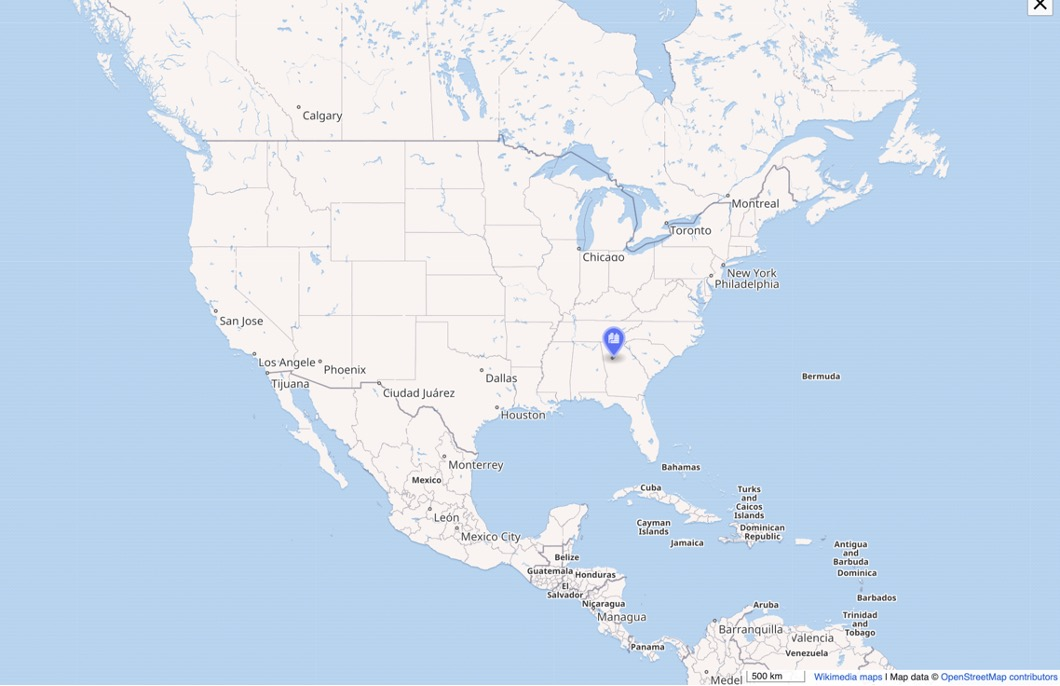
\includegraphics[width=1\textwidth]{map2/location.jpg}
\caption{Figure 1: Different levels of urban development intensity}
\label{fig:figure1}
\end{center}
\end{figure}

\begin{center}
\centering
Figure 1: Project Location on Planet Earth
\end{center}


\subsection{Terms and Context}
Metal Music: A music genre, originated in the UK and US in the late 60s and early 70s. It evolved from blues rock, psychedelic rock, and acid rock, and is known for its powerful sound featuring distorted guitars, long guitar solos, strong beats, and high volume. Metal music lovers are called "metalheads"(Walser, 1993), which is the major consumer of metal music venue business.

Music Venue: A music venue is any location used for a concert or musical performance. Music venues range in size and location, from a small coffeehouse for folk music shows, an outdoor bandstand or a concert hall to an indoor sports stadium.  In this project, the music venue is in the same scope yelp's music venue category.


\subsection{Conceptual Vision and Model}
The conceptual model, which includes spatial and mathematical components, converts transport and demographic factors into measurable metrics. These metrics are represented by scores, and then joined by location, using the area as a weight to aggregate scores for neighborhoods. The neighborhoods with the highest scores are then selected, and restriction layers are applied to determine the most suitable ones. The final step is identifying and conducting a detailed analysis of the neighborhood that is most suitable for a metal music venue business.

\subsection{Objectives}
The objectives of this project are to:
\begin{enumerate}
\item{Evaluate the accessibility to current music venues.}
\item{Identify neighborhoods with high potential for establishing metal music venues, considering transport, demographic, and urban planning factors.}
\item{Contribute to the promotion of a vibrant music scene in Atlanta.}
\end{enumerate}

\section{Data Processing and Inclusion}

\subsection{Data Source}

\textbf{Atlanta Statistical Neighborhood}

City of Atlanta Neighborhood Area polygon data were derived from the course materials provided in Lab 2.

\textbf{Music Venue Point of Interest}
Points of interest for music venues were obtained through query from the Yelp Business Search API(Yelp, 2023). 

\textbf{Demographic Data: Census Tract} The author focused on Atlanta, situated within Fulton and DeKalb counties. The author sourced polygon data from the American Community Survey (ACS) 5-year estimates in 2019 (U.S. Census Bureau, 2019). This data included monthly housing prices, median household income, median age, and racial distribution. The housing prices offered insight into the rental costs for music venues, while the median household income and age highlighted the consumer characteristics of the neighborhood.

\textbf{Demographic Data: Metalheads’ Demography} 
Shukla’s 2022 sociology paper provided the age, gender, and racial distribution data of metalheads(Shukla,2022).

\textbf{Transport Data: Road Network and Parking Lots} 
The author used a Python query with OSMnx (Boeing, 2017) to download the road network polylines and parking lot data(points and polygons) for Atlanta, the retrieving time stamp is November 21st, 2023.

\textbf{Urban Planning Data: Zoning and Livable Center Initiative}
Zoning and Livable Center Initiative(LCI) are directly downloaded from fulton county GIS data portal(Fulton County, 2023).

\begin{figure}[H]
\begin{center}
\centering
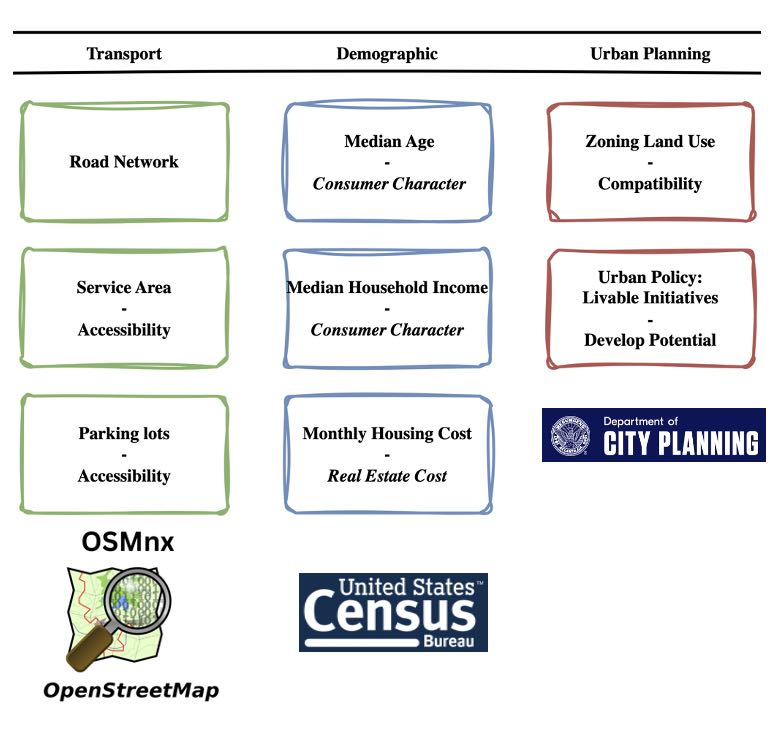
\includegraphics[width=0.3\textwidth]{diagram/data.jpg}
\caption{Data source and Usage}
\label{fig:figure1}
\end{center}
\end{figure}

\begin{center}
\centering
Figure 2: Data source and Usage
\end{center}


\subsection{Data Accuracy}

This project acknowledges several potential sources of inaccuracies in the data. The OSMnx data, derived from GPS, may exhibit meter-level inaccuracies due to daily variations in accuracy and systematic errors. Additionally, naming inaccuracies may exist (OpenStreetMap Wiki, 2020). The Yelp Business Search API, which returns up to 1000 businesses and excludes businesses without reviews, may not account for some music venues that lack reviews or exceed the limit (Yelp, 2023). Furthermore, the demographic data of metalheads, researched in England, may not fully apply to Atlanta due to differing cultural and historical contexts.

The first two inaccuracies are disregarded as this project operates at the neighborhood level. The potential demographic inaccuracy is mitigated by focusing solely on age distribution, excluding race and gender considerations.

To bolster accuracy, this project utilizes 5-year estimates from the ACS, rather than 1-year estimates. This approach enhances statistical reliability by drawing on a larger data set (U.S. Census Bureau, 2019).

\subsection{Data Processing}

Before integrating data into the spatial model, two crucial steps are executed. The initial step involves transforming the coordinate reference system to WGS 84 UTM Zone 16. The subsequent step entails conducting a service area analysis in the network. In ArcGIS Pro, music venue points of interest serve as facilities, with time thresholds set at 5, 10, 15, and 20 minutes, and driving designated as the network type (Gutiérrez, 2008).

\begin{figure}[H]
\begin{center}
\centering
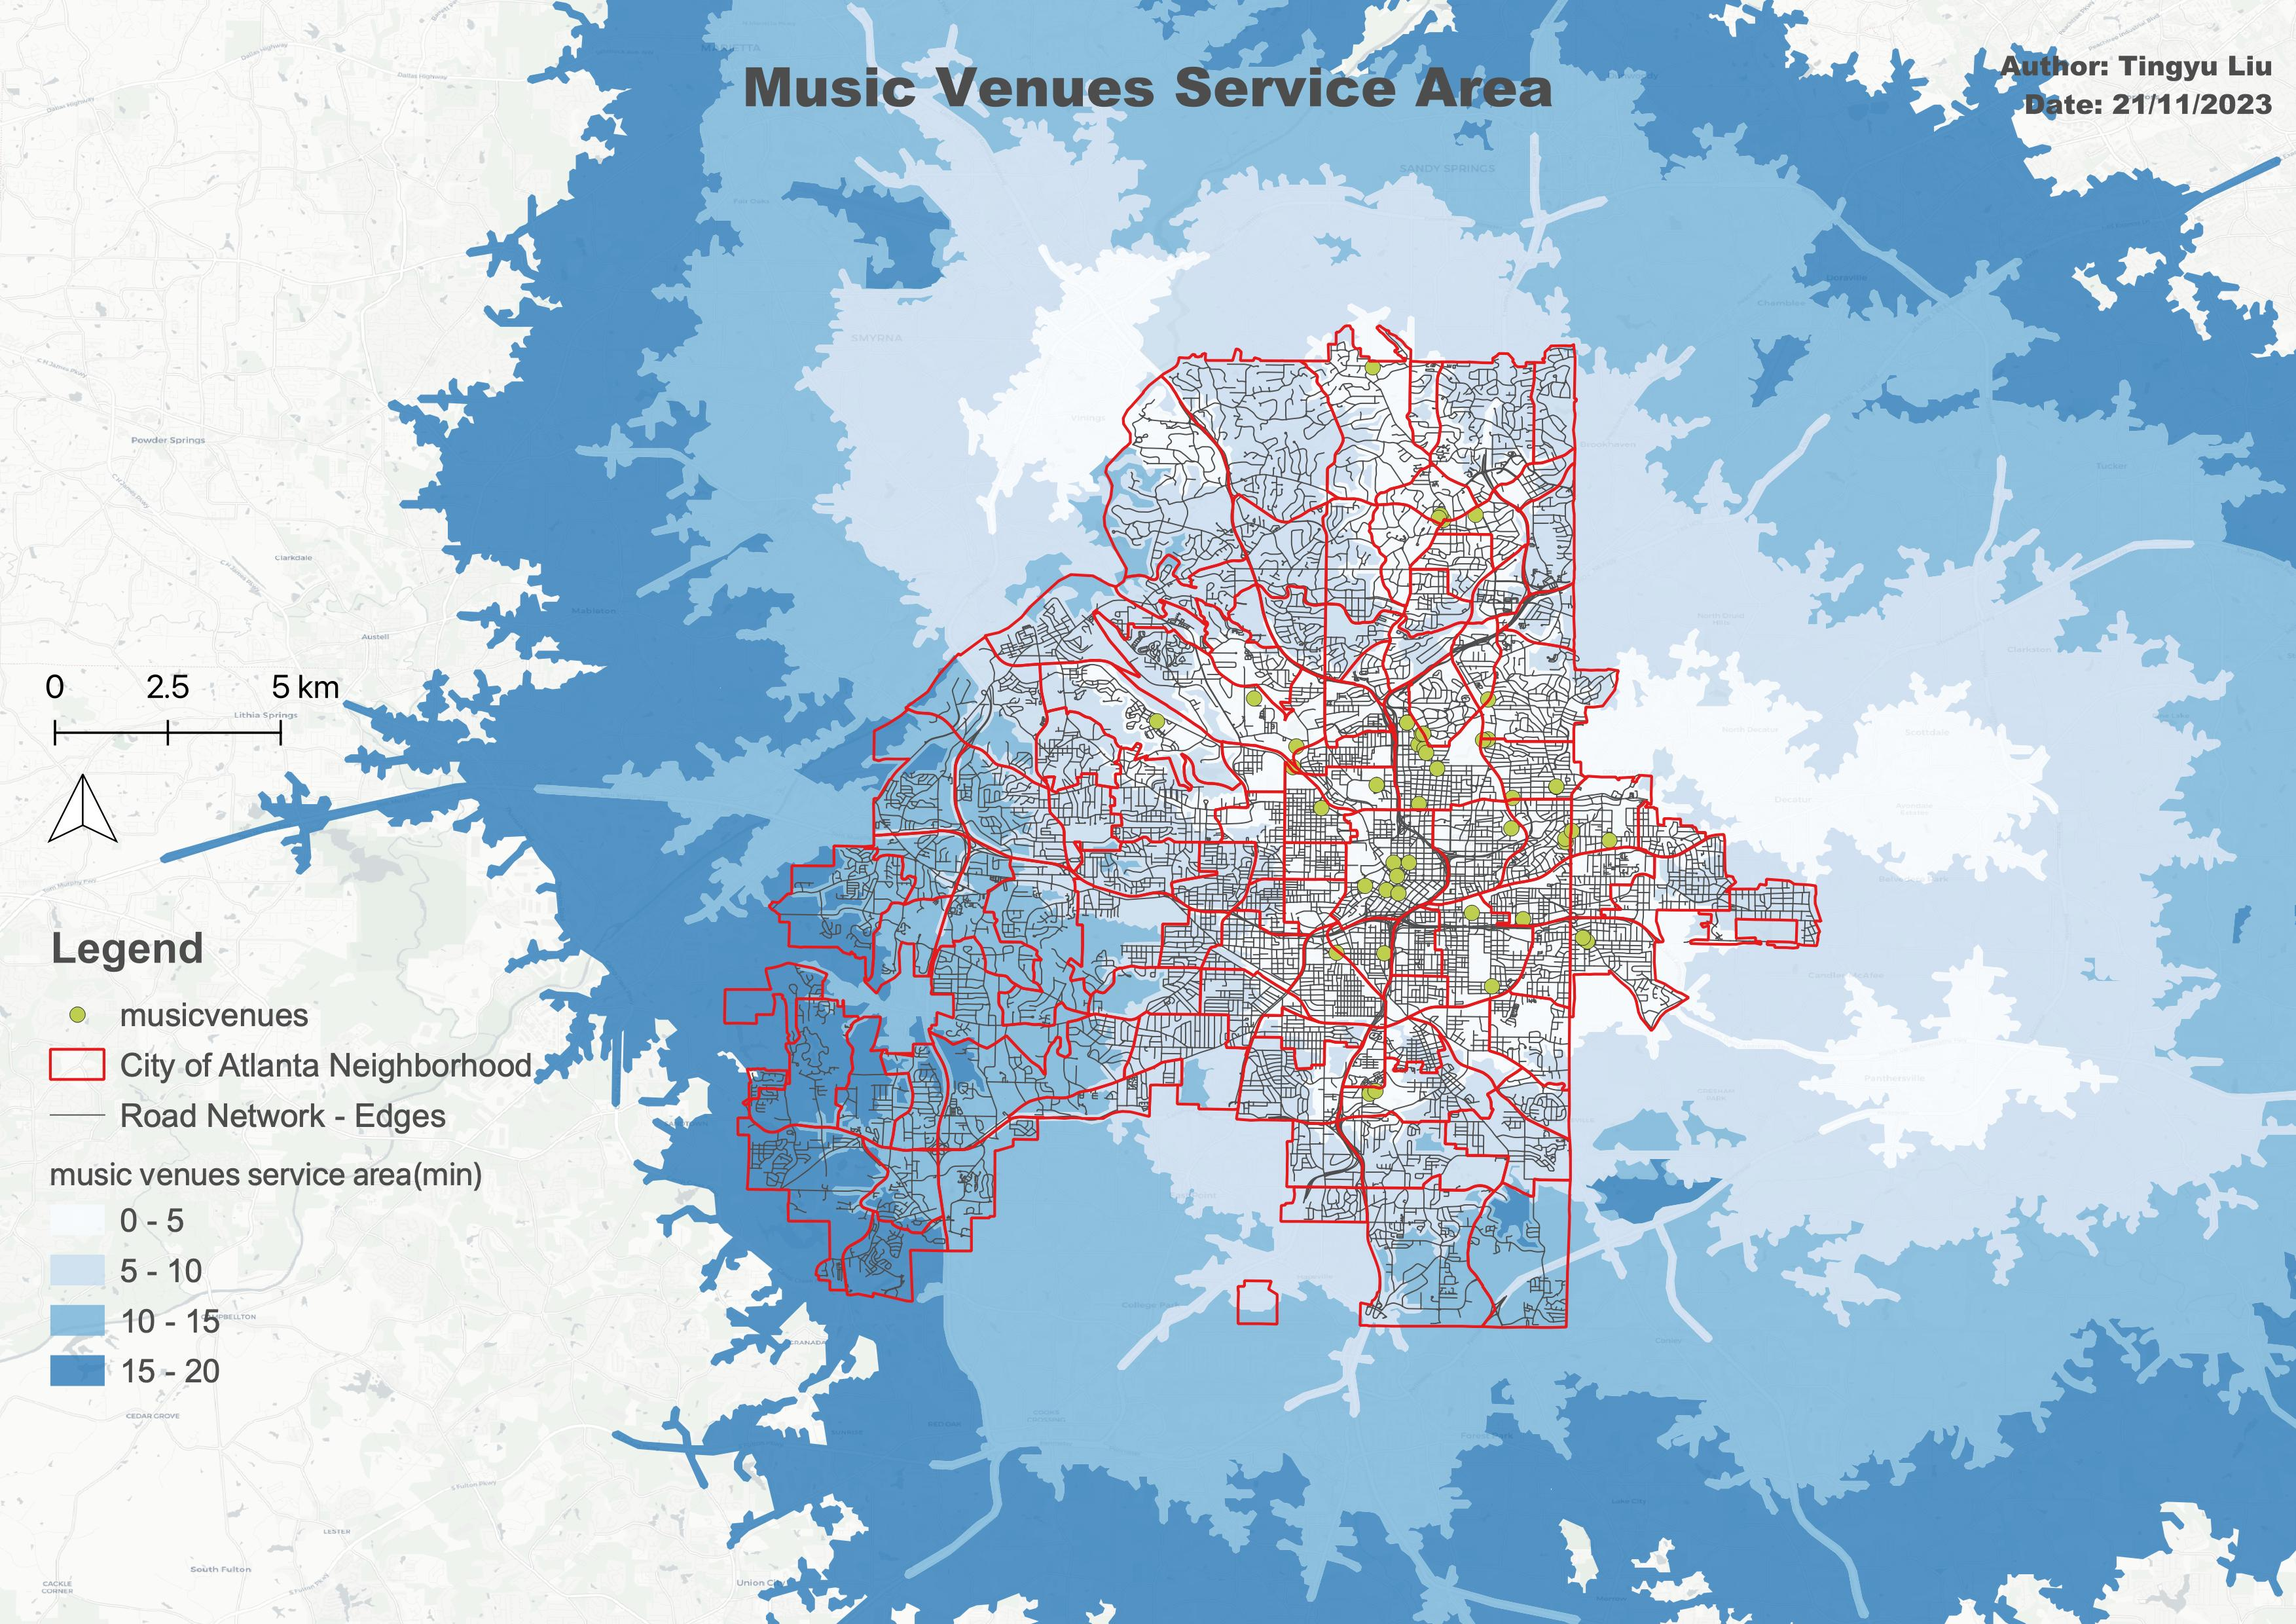
\includegraphics[width=1\textwidth]{map2/2_serviec_area.jpg}
\caption{Figure 1: Different levels of urban development intensity}
\label{fig:figure1}
\end{center}
\end{figure}

\begin{center}
\centering
Figure 3: Music Venue Service Area
\end{center}





\section{Solution and Methods}
\subsection{Spatial and Mathematical Model}
The spatial and mathematical model involved building a spatial model to convert transport and demographic factors to quantifiable metrics, then ranking neighborhoods based on these metrics to find the top 5 neighborhood candidates. Then, urban planning and transport factors were used as restrictions to select the best suitable one.


\begin{figure}[H]
\begin{center}
\centering
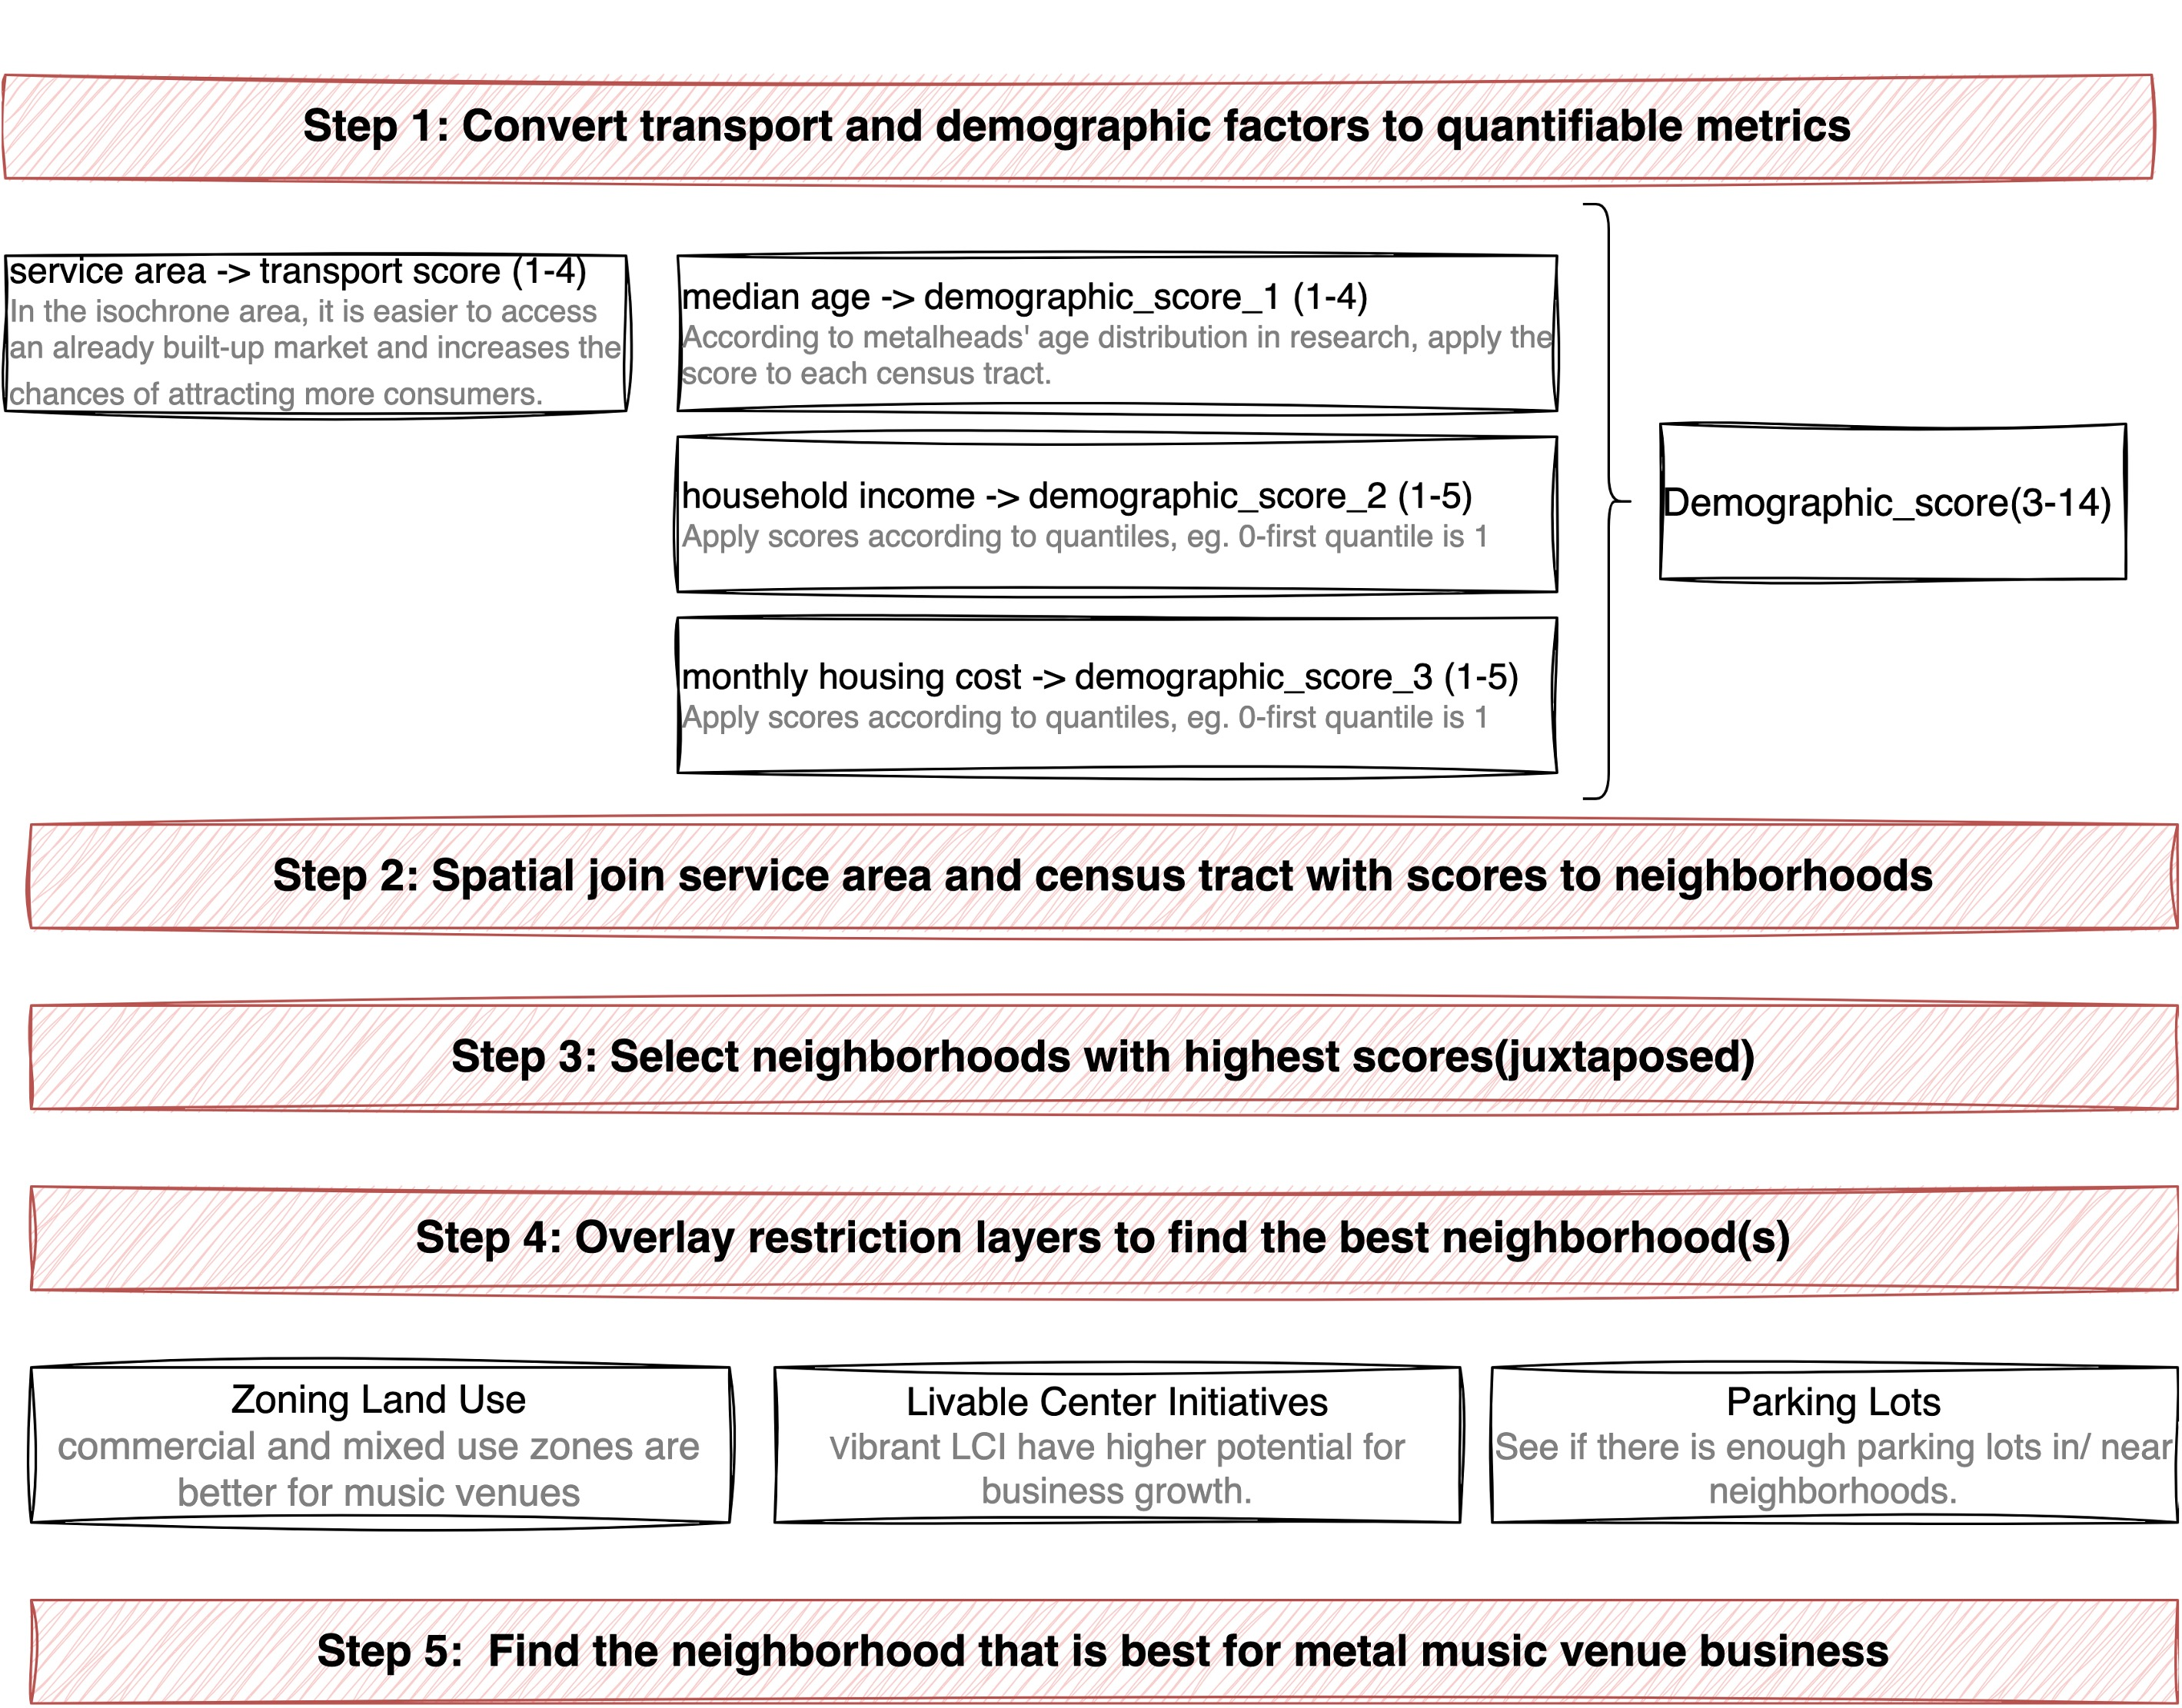
\includegraphics[width=0.9\textwidth]{diagram/model.jpg}
\caption{Figure 1: Different levels of urban development intensity}
\label{fig:figure1}
\end{center}
\end{figure}

\begin{center}
\centering
Figure 4: Model Steps
\end{center}

\subsection{Model Steps}


\textbf{1. Convert transport and demographic factors to quantifiable metrics.}\\
In the transport factor (network analysis), scores were applied based on accessibility to existing music venues. A higher score indicated shorter driving time to existing music venues. According to economic geography, concentration is beneficial for the music venue business. More accessible places are more familiar to current metalheads, making it easier to build cultural recognition. For instance, a service area within 0-5 minutes driving received a score of 4 out of 4.

In terms of age distribution, the author applied scores to each census tract based on the age distribution of metalheads from the research. A higher score indicated a more similar range to the metalheads’ age range. For example, the age range of 25-35 received a score of 4 out of 4.


\begin{figure}[H] 
    \centering
    \subfloat{%
        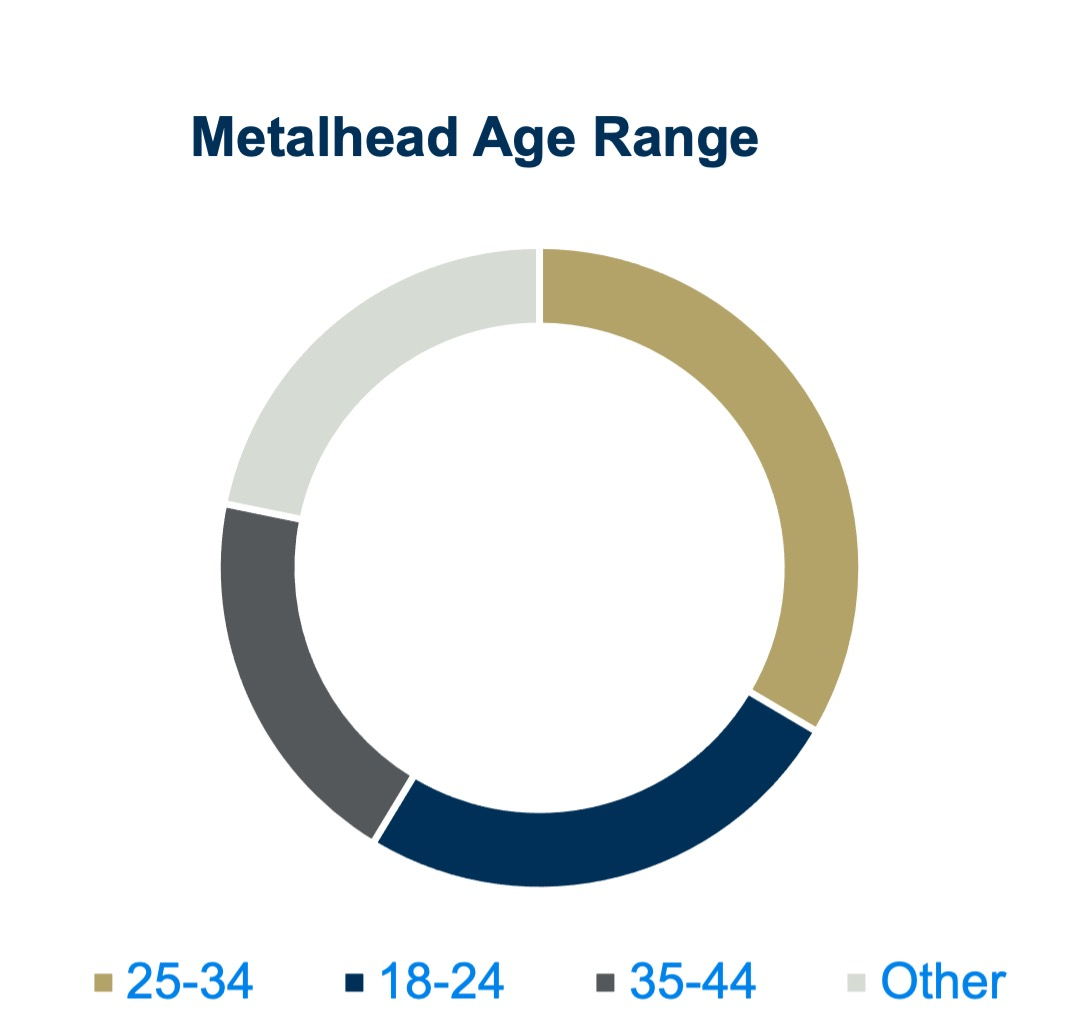
\includegraphics[width=0.48\textwidth]{map2/pie.jpg}%
        \label{fig:a}%
        }%
    \hfill%
    \subfloat{%
        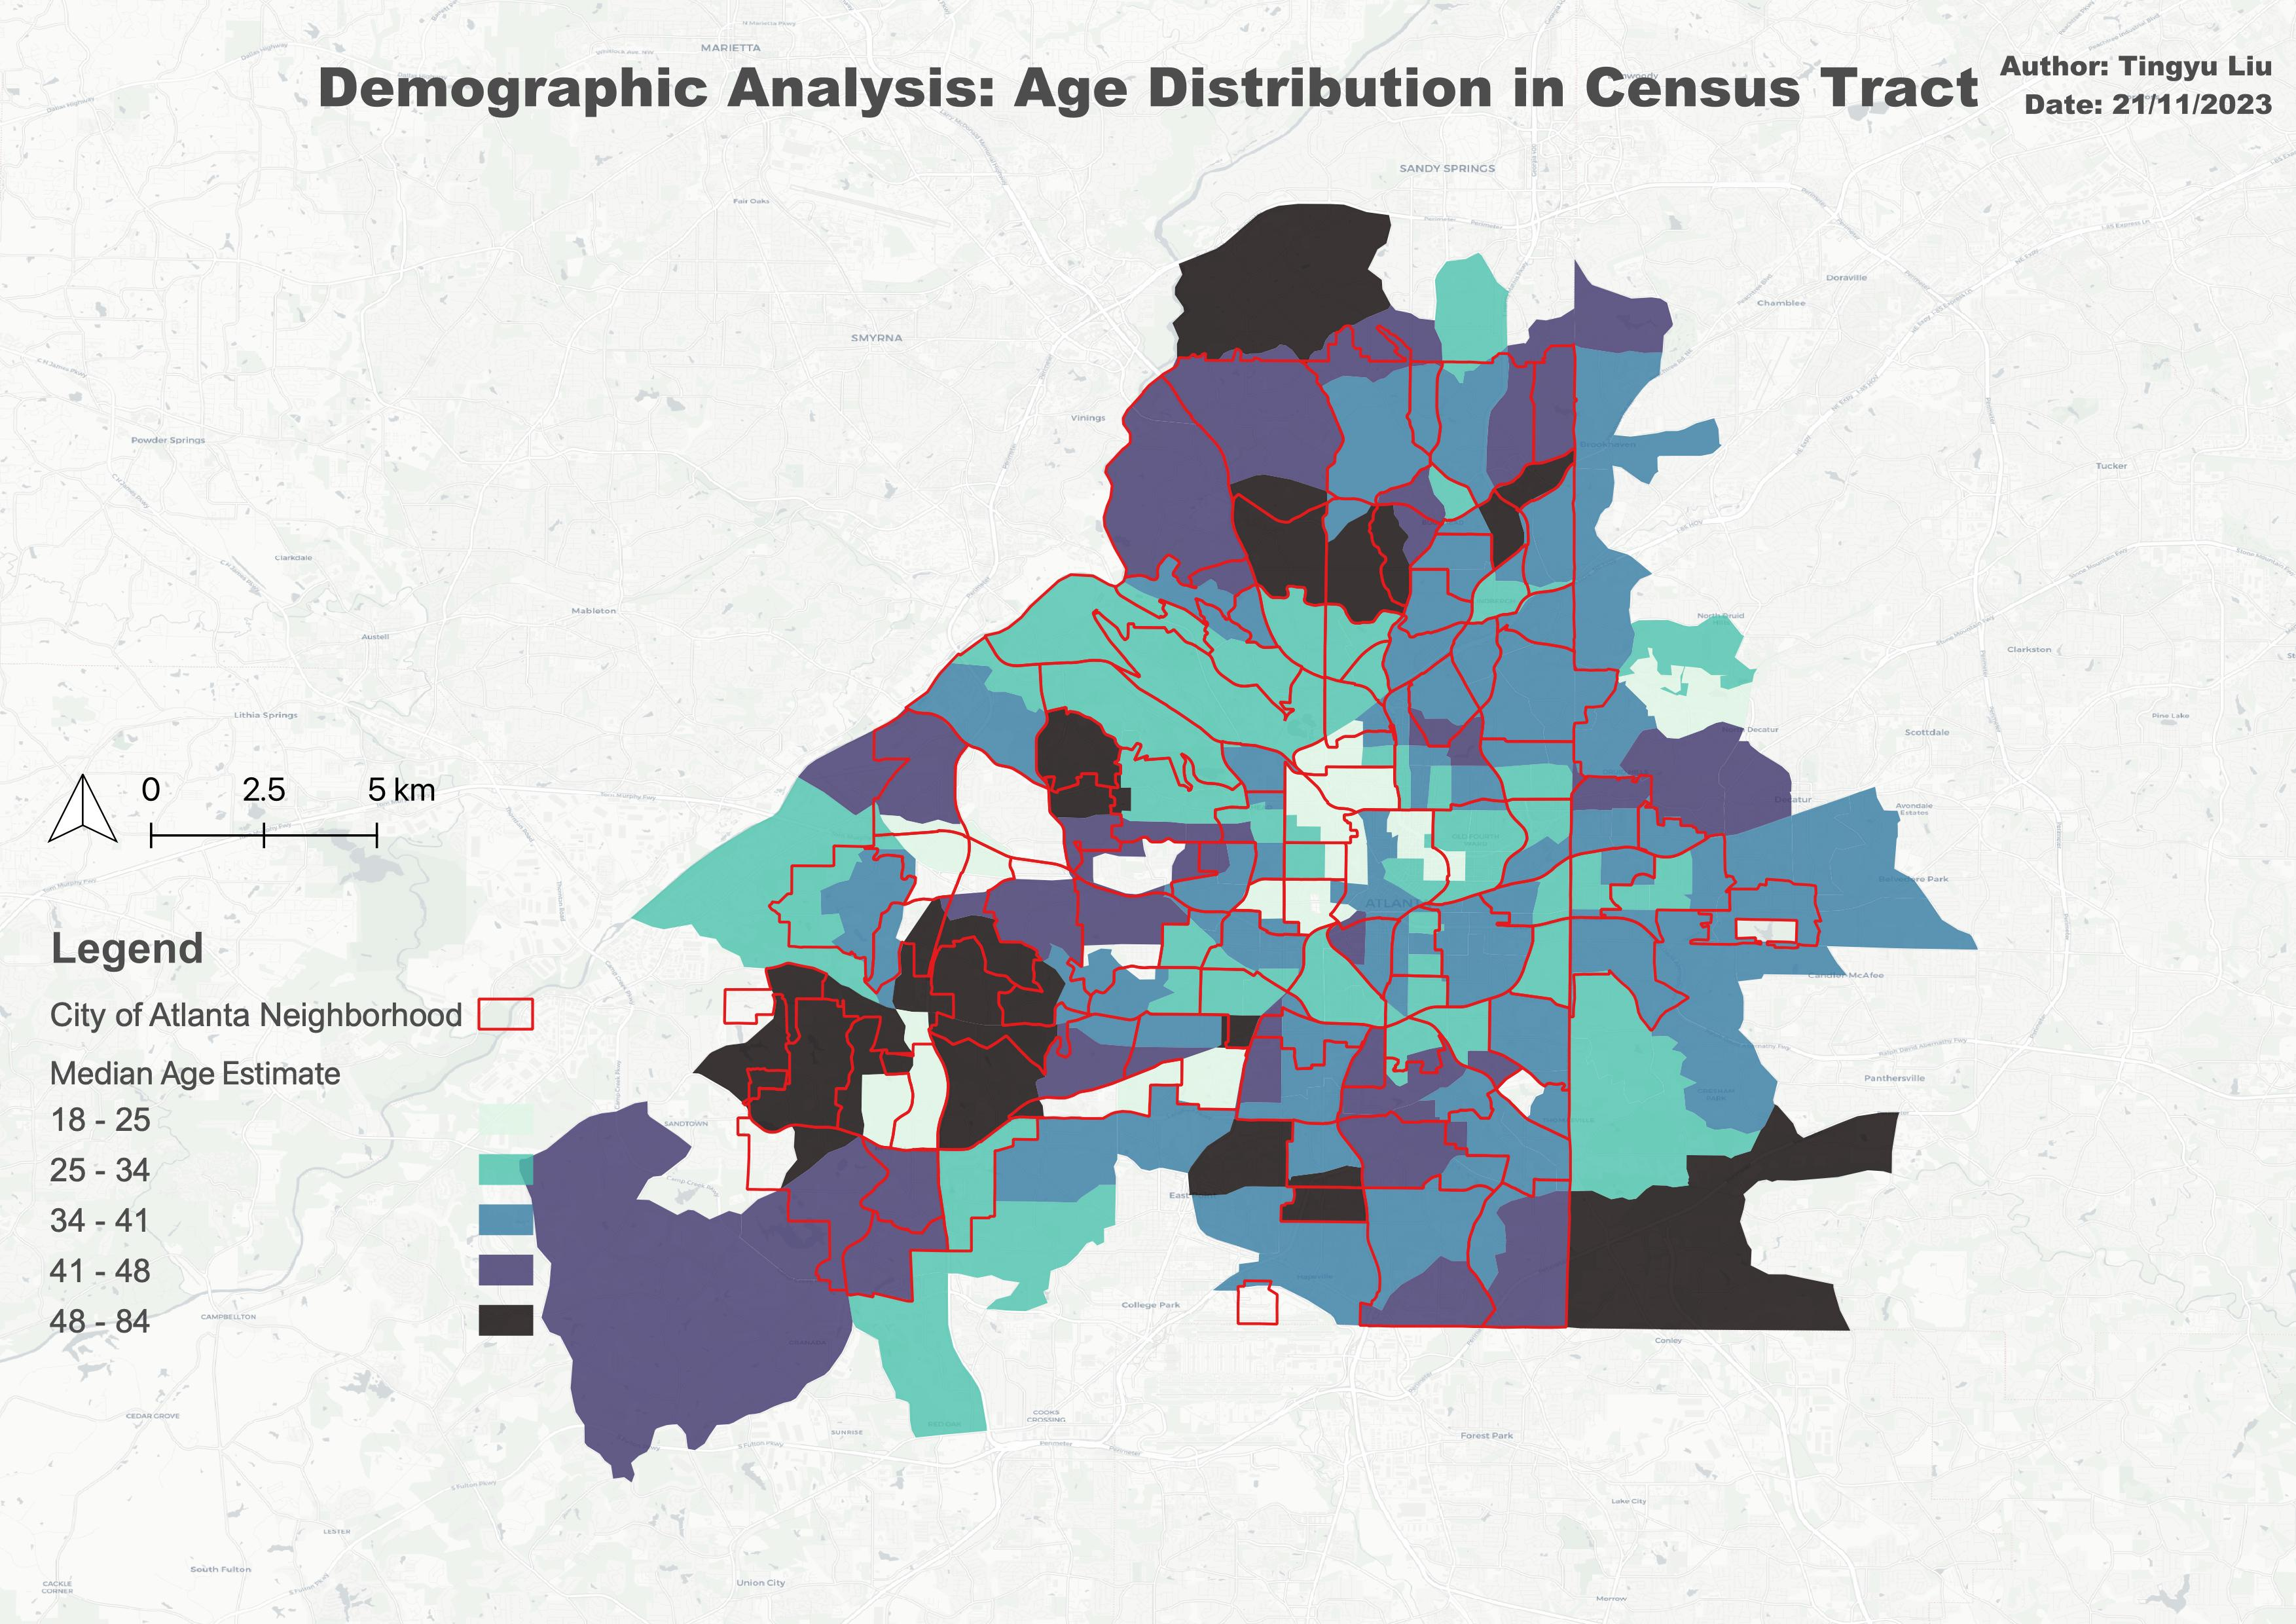
\includegraphics[width=0.48\textwidth]{map2/3_age.jpg}%
        \label{fig:b}%
        }%
    \caption{all the data}
\end{figure}

\begin{center}
\centering
Chart 1: Metalhead's age  \& Figure 5: Demographic Analysis: Age Spatial Distribution
\end{center}

In the median household income, the author separated income into 5 ranges according to equal quantile and applied scores according to quantiles. A higher score indicated higher consuming capacity. For example, an income range of 102303 - 208750 dollars received a score of 5 out of 5.

In monthly housing cost, the author separated income into 5 ranges according to equal quantile and applied scores according to quantiles. A higher score indicated higher consuming capacity. For example, a monthly housing cost range of 1657 - 2761 dollars received a score of 5 out of 5.


\begin{figure}[H] 
    \centering
    \subfloat{%
        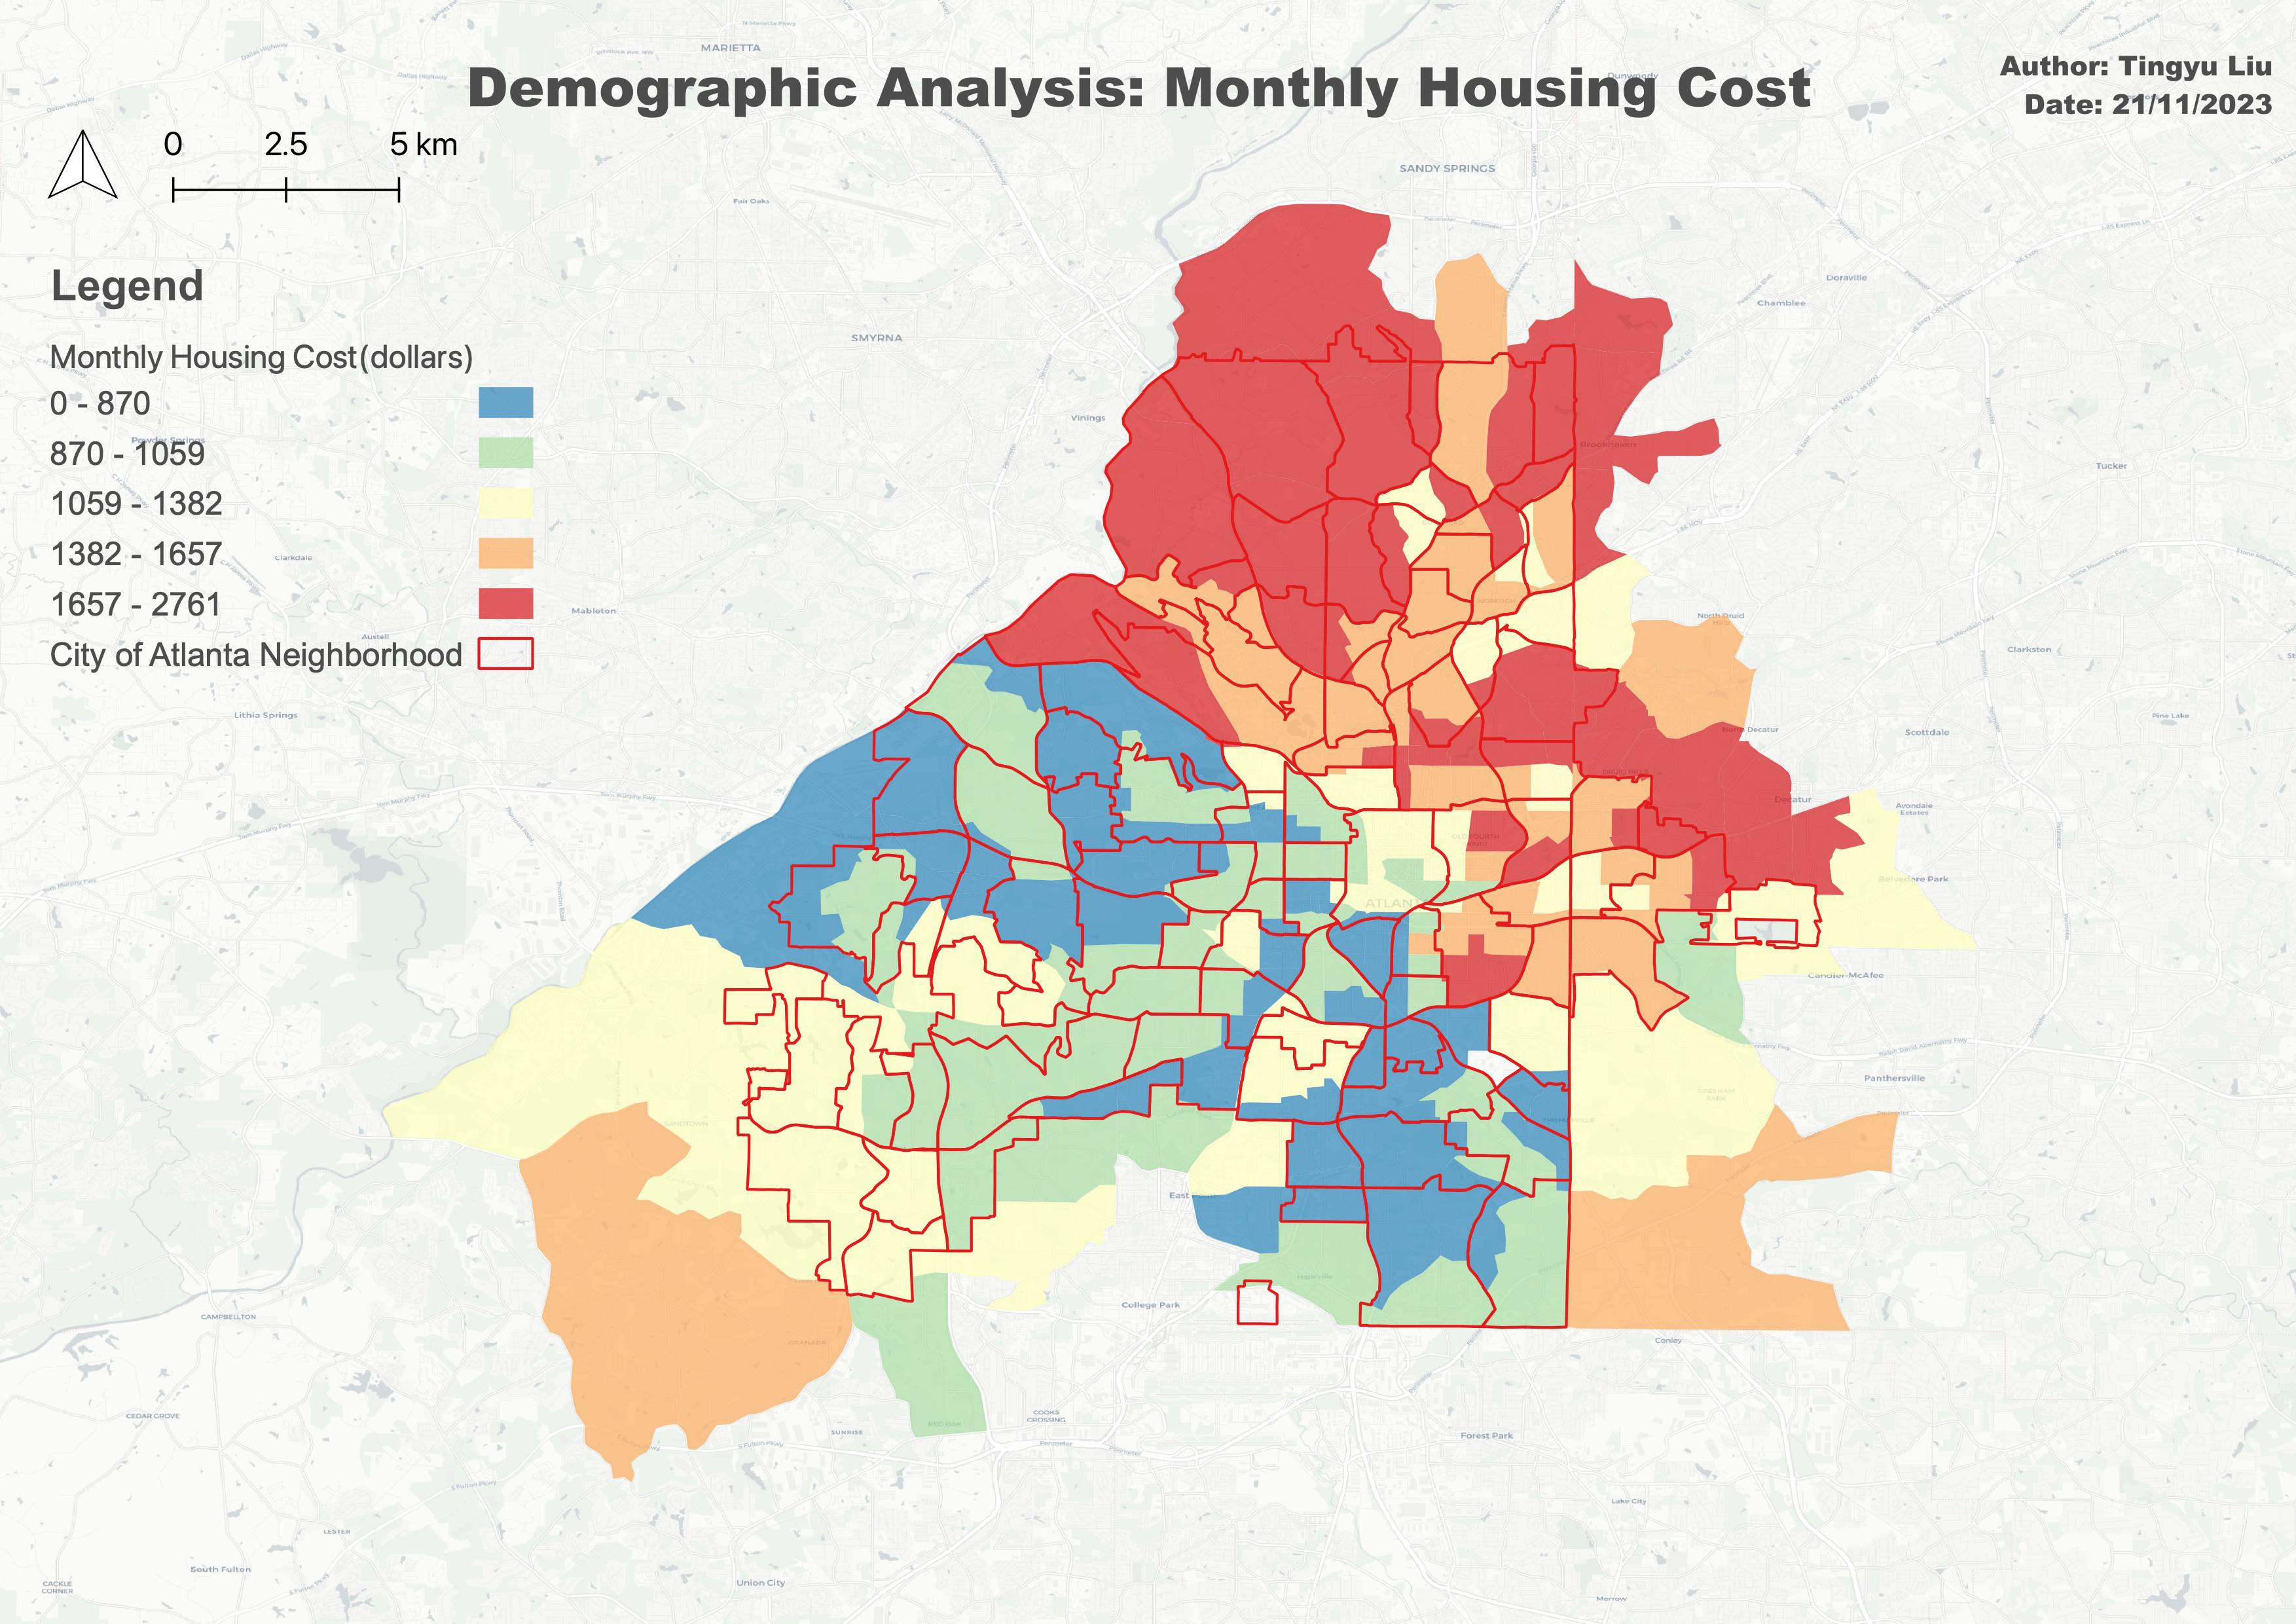
\includegraphics[width=0.48\textwidth]{map2/3_monthly housing cost.jpg}%
        \label{fig:a}%
        }%
    \hfill%
    \subfloat{%
        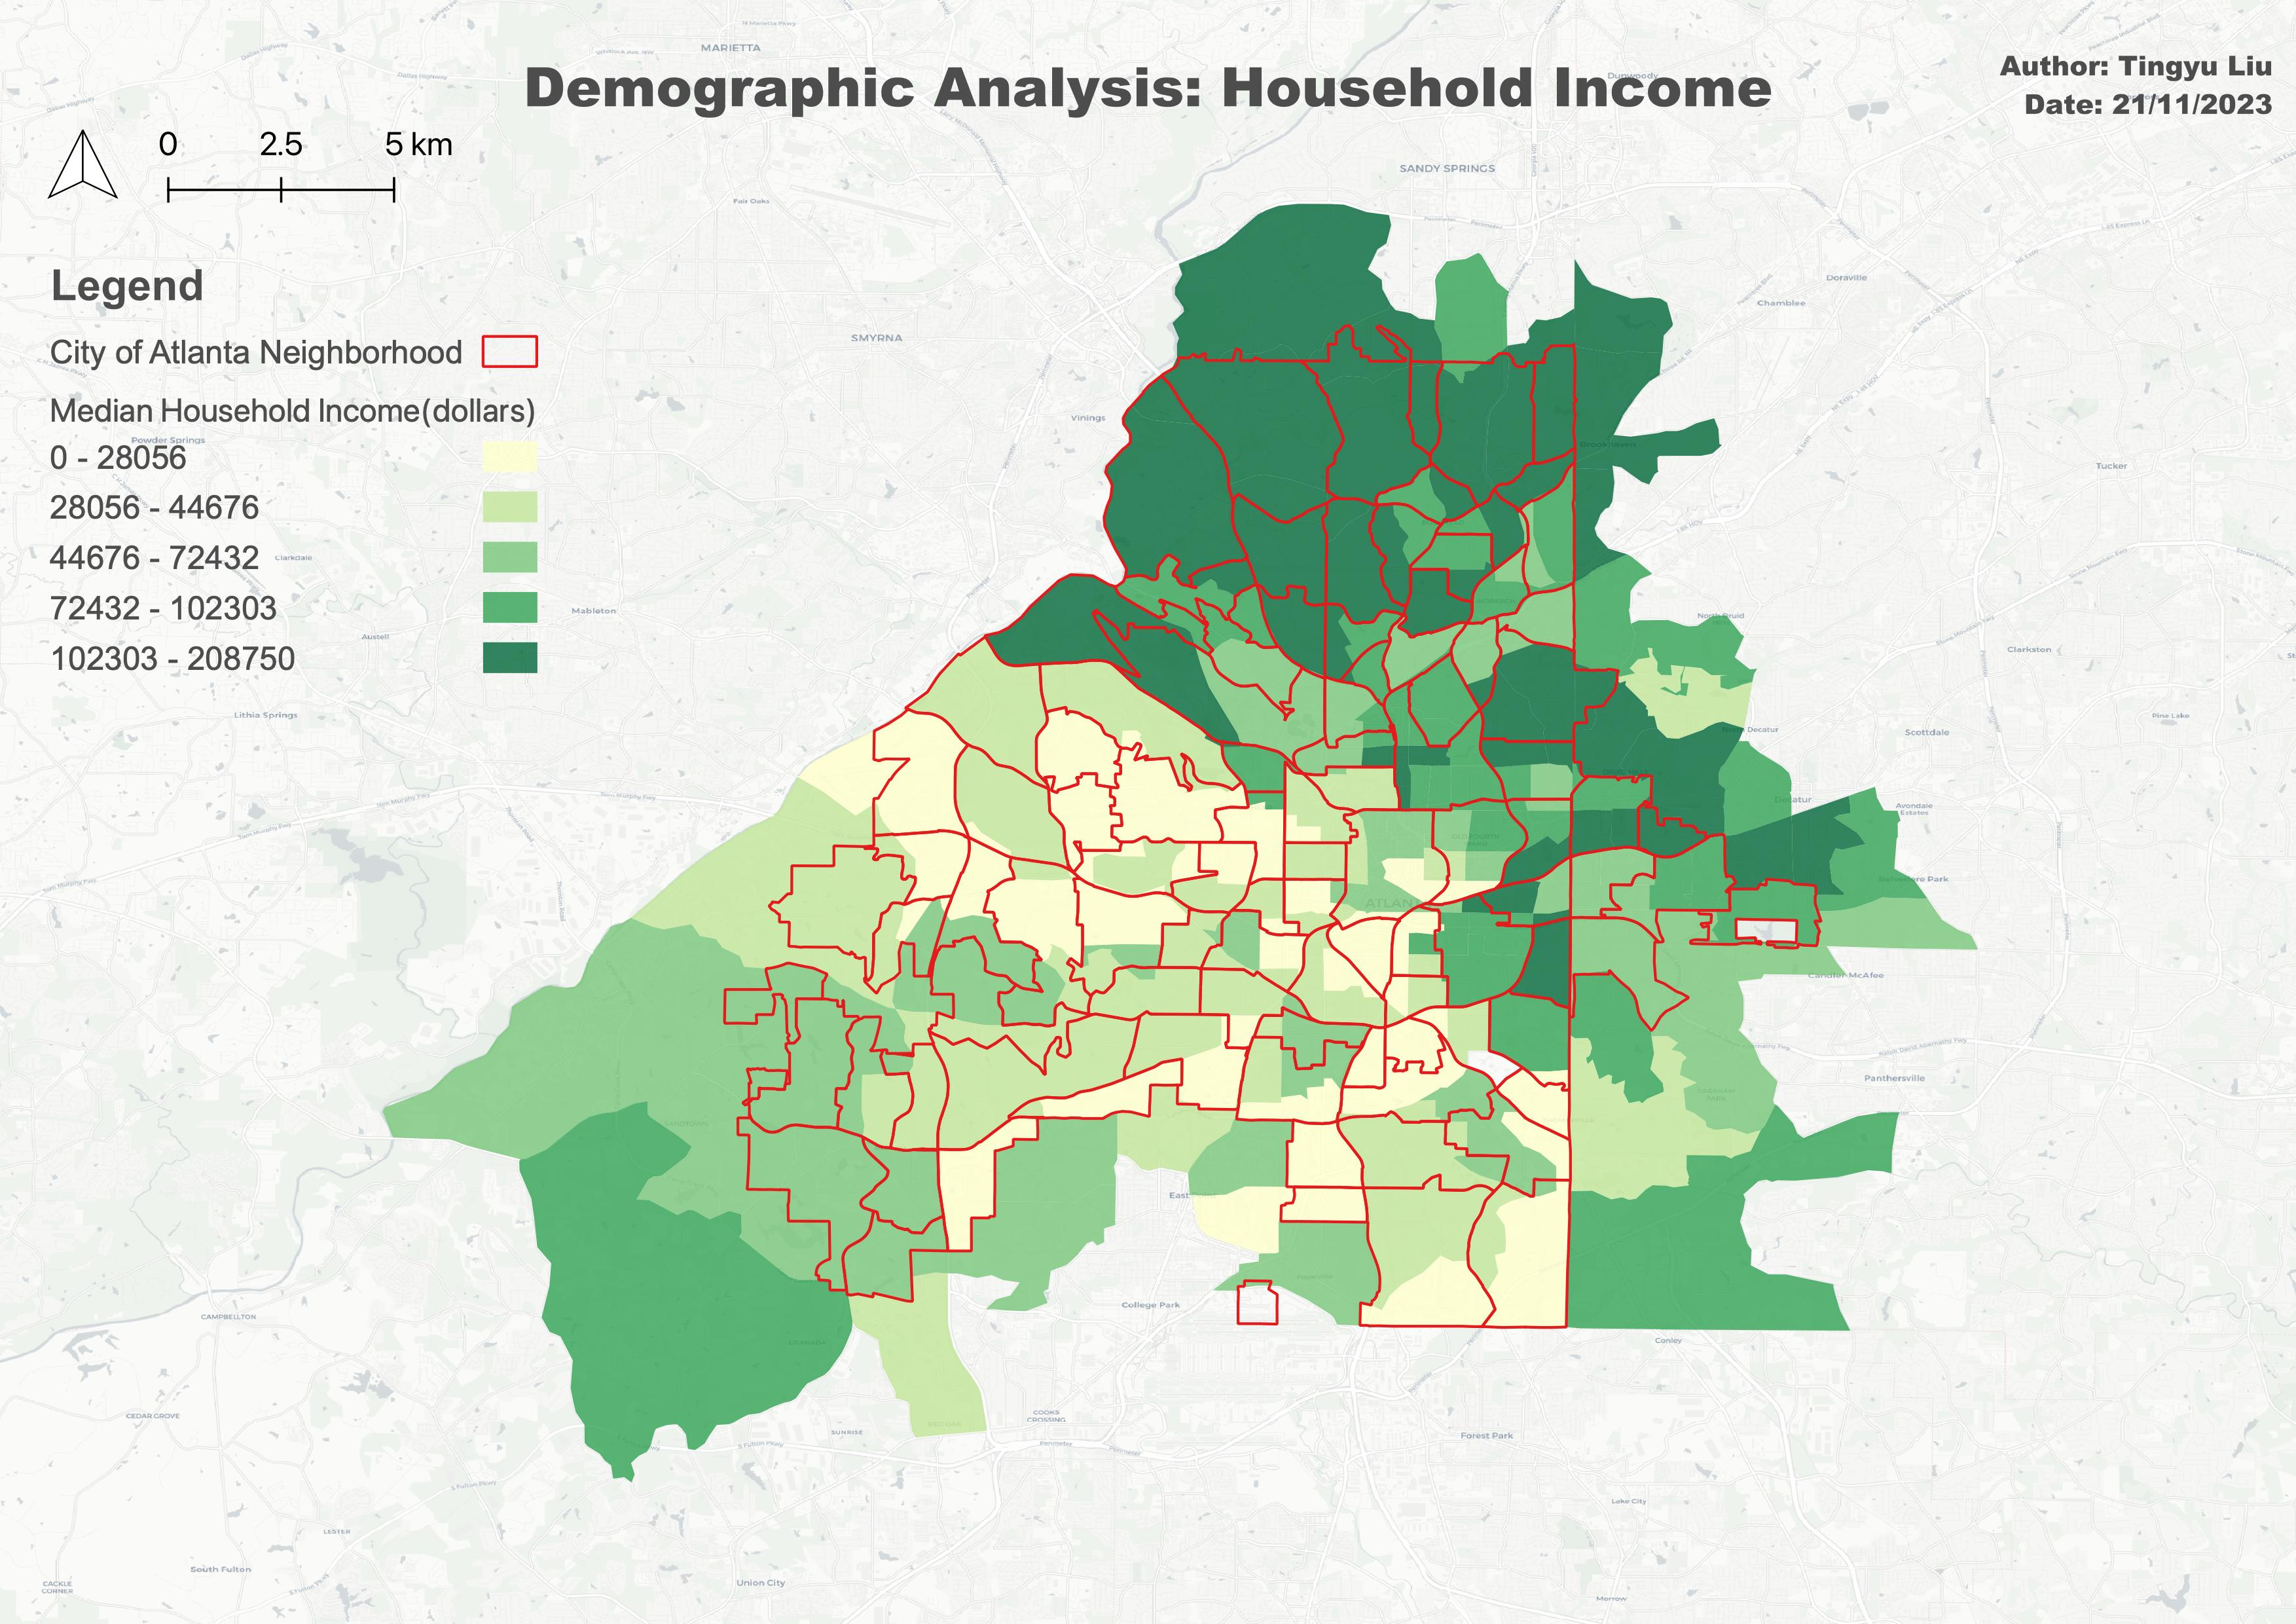
\includegraphics[width=0.48\textwidth]{map2/3_income.jpg}%
        \label{fig:b}%
        }%
    \caption{all the data}
\end{figure}

\begin{center}
\centering
Figure 6: Demographic Analysis: Housing Cost \& Figure 7: Demographic Analysis: Household Income
\end{center}


\textbf{2. Spatial join service area and census tract with scores to neighborhoods\\}
In the first steps, the scores are in the service area polygons or census tract polygon, and considering the objective is to find out the best neighborhood, so the author join score attribute by location, and sum the score in each neighborhoods based on area.\\
In the initial stages of the process, each service area polygon or census tract polygon is assigned a score, denoted as $S_i$, where $i$ represents the index of the polygon. The objective is to identify the optimal neighborhood, which necessitates the aggregation of scores by location. This is achieved by associating the score attribute with each neighborhood. The total score, $T_j$, for a given neighborhood $j$, is computed by summing the scores of all polygons within the neighborhood, each weighted by their respective area, $A_i$. Mathematically, this can be represented as:

\begin{equation}
T_j = \sum_{i \in N_j} \frac{A_i}{A_{neighborhood}} \cdot S_i
\end{equation}

Here, $N_j$ signifies the set of polygons within neighborhood $j$, and $A_{total}$ is the total area of all polygons. This equation effectively calculates the weighted scores in each neighborhood based on area, aligning with the described procedure.


\textbf{3. Select neighborhoods with highest scores(juxtaposed)\\}
After summarying up the score to neighborhood, sort final score in descending order, and select the neighborhood that has top score.


\textbf{4. Overlay restriction layers to find the best neighborhood(s)}
The author consider two restrictions: urban planning(zoning and LCI) and transport(parking lot).  

Land use designated for commercial and mixed-use purposes aligns more effectively with the operational requirements of a music venue business. Furthermore, the LCI(Livable Centers Initiative), which advocates for the creation of vibrant, walkable spaces, provides additional support for these neighborhoods as potential locations for the proposed music venue. The more ratio of commercial and mixed-use area, and the more overlay with LCI, the more suitable for music venue business for a neighborhood.

Metal music events usually occur during the evening hours((Walser, 1993), leading to a majority of the audience opting to drive to the venue. To cater to this demographic, music venues typically undertake one of two strategies. They either allocate substantial financial resources towards the acquisition of a parking lot, or they strategically select a location in close proximity to public parking facilities. 

\textbf{5. Find the neighborhood that is best for metal music venue business}


\subsection{Integration of Tools and Methods} The author integrated various tools and methods in this study. ArcGIS Pro was used for the Network Analyst (Service Area), and QGIS was used for Layout, Join Attribute by Location, Field Calculator, and Attribute Table. Additionally, Python packages OSMNX, Folium, and Geopandas were used for geo-spatial data collection, processing, and interactive visualization. 

\section{Research Results, Discussion, and Conclusion}
\subsection{Analysis Result}

\textbf{Competitor Analysis}

The competitor analysis focuses on the existing music venues in the city of Atlanta, which could potentially pose as business competitors for new metal music venues. This analysis involves examining the spatial distribution of existing music venues, their attributes, and their kernel density.

A significant concentration of music venues is found in mid-eastern Atlanta, demonstrating the economic geography concept of clustering (Florida et al., 2010). Clustering of related businesses can reduce production costs due to competition among suppliers and increased specialization. Interestingly, even same-sector firms can benefit from clustering by attracting more suppliers and customers than they could individually.

\begin{figure}[H] 
    \centering
    \subfloat{%
        \includegraphics[width=0.48\textwidth]{map2/1_competitor.jpg}%
        \label{fig:a}%
        }%
    \hfill%
    \subfloat{%
        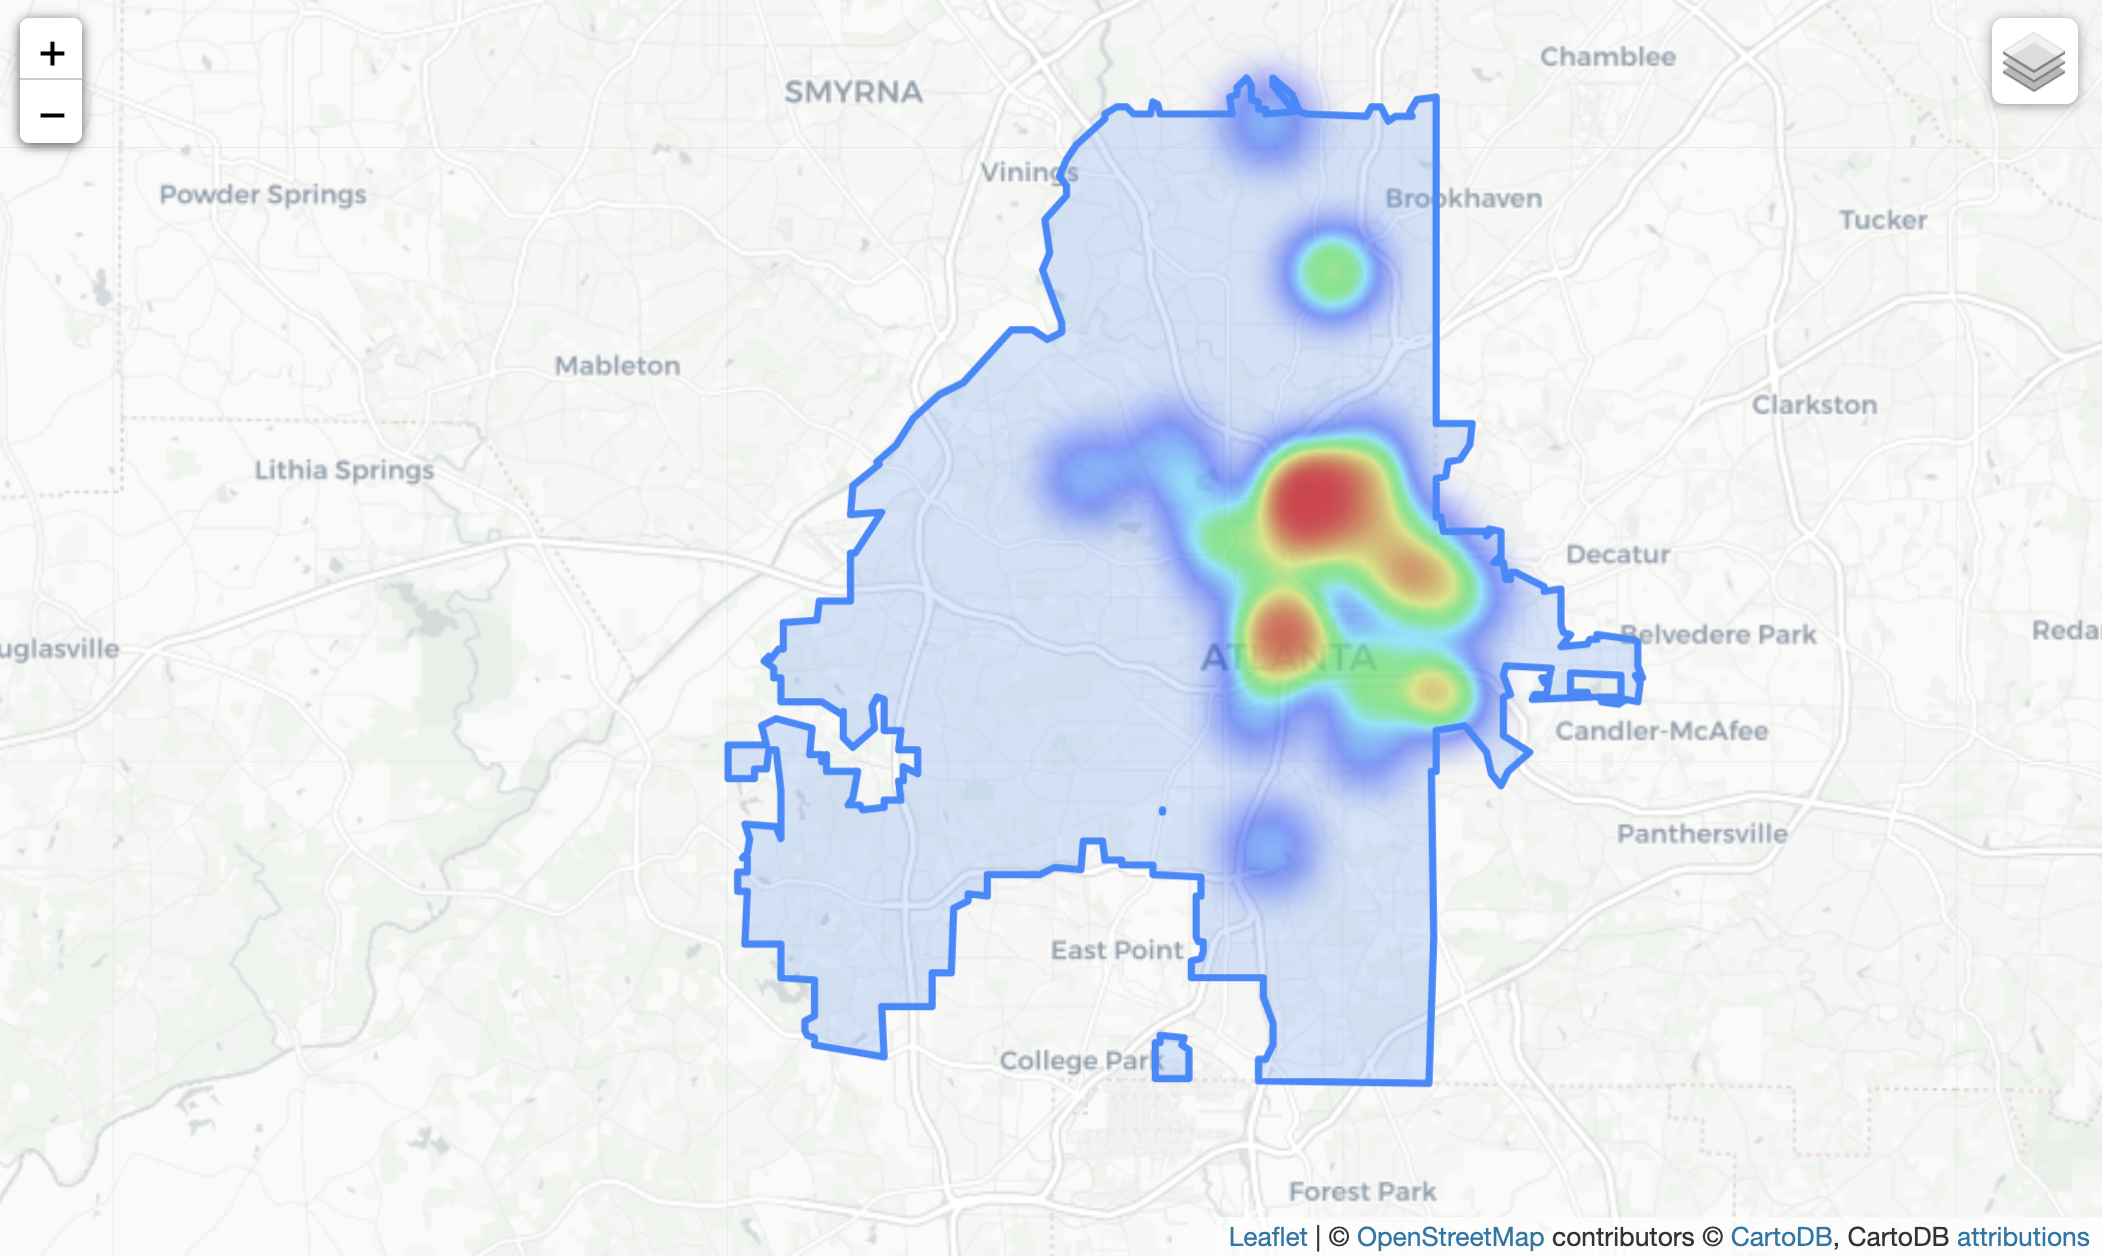
\includegraphics[width=0.48\textwidth]{map2/heatmap.png}%
        \label{fig:b}%
        }%
    \caption{all the data}
\end{figure}


\begin{center}
\centering
Figure 8: Neighborhood Music Venue Count \& Figure 9: Music Venue Kernel Density
\end{center}



\textbf{Transport Analysis}

The transport analysis is service area in network analysis, which evaluate the accessibility of existing music venues. 

Midtown, distinguished by the highest number of music venues, exhibits a spatial distribution primarily on the eastern side of Atlanta. Neighborhoods with a significant concentration of music venues, such as Midtown, Castleberry Hill, and Akins Park, are centrally located, forming a cluster in the central part of the city.

The areas with the greatest accessibility, defined as those within a 0-5 minute driving time, display a spatial skew when compared to the distribution of music venues. While the music venues are predominantly distributed along an east-west axis, the service area extends more significantly in the north-south direction. This pattern can be largely attributed to the presence of the I-75 and I-85 highways. The influence of transport factors on accessibility and location analysis is evident. Music venues within a shorter driving time achieve higher transport scores, indicating that the proximity to major highways and ease of access are beneficial for the music venue business.

\textbf{Demographic Analysis}

The neighborhoods exhibiting the highest demographic suitability for music venues, in terms of demographic features, are predominantly located on the north and east side of the city of Atlanta. A comparison with the distribution of music venues reveals that the downtown area, despite having a lower demographic score, houses several music venues. This observation underscores the importance of considering transport features, specifically the service area, as it represents existing accessibility. The presence of music venues in areas with lower demographic scores suggests that accessibility may play a significant role in the location of these venues.

\begin{figure}[H] 
    \centering
    \subfloat{%
        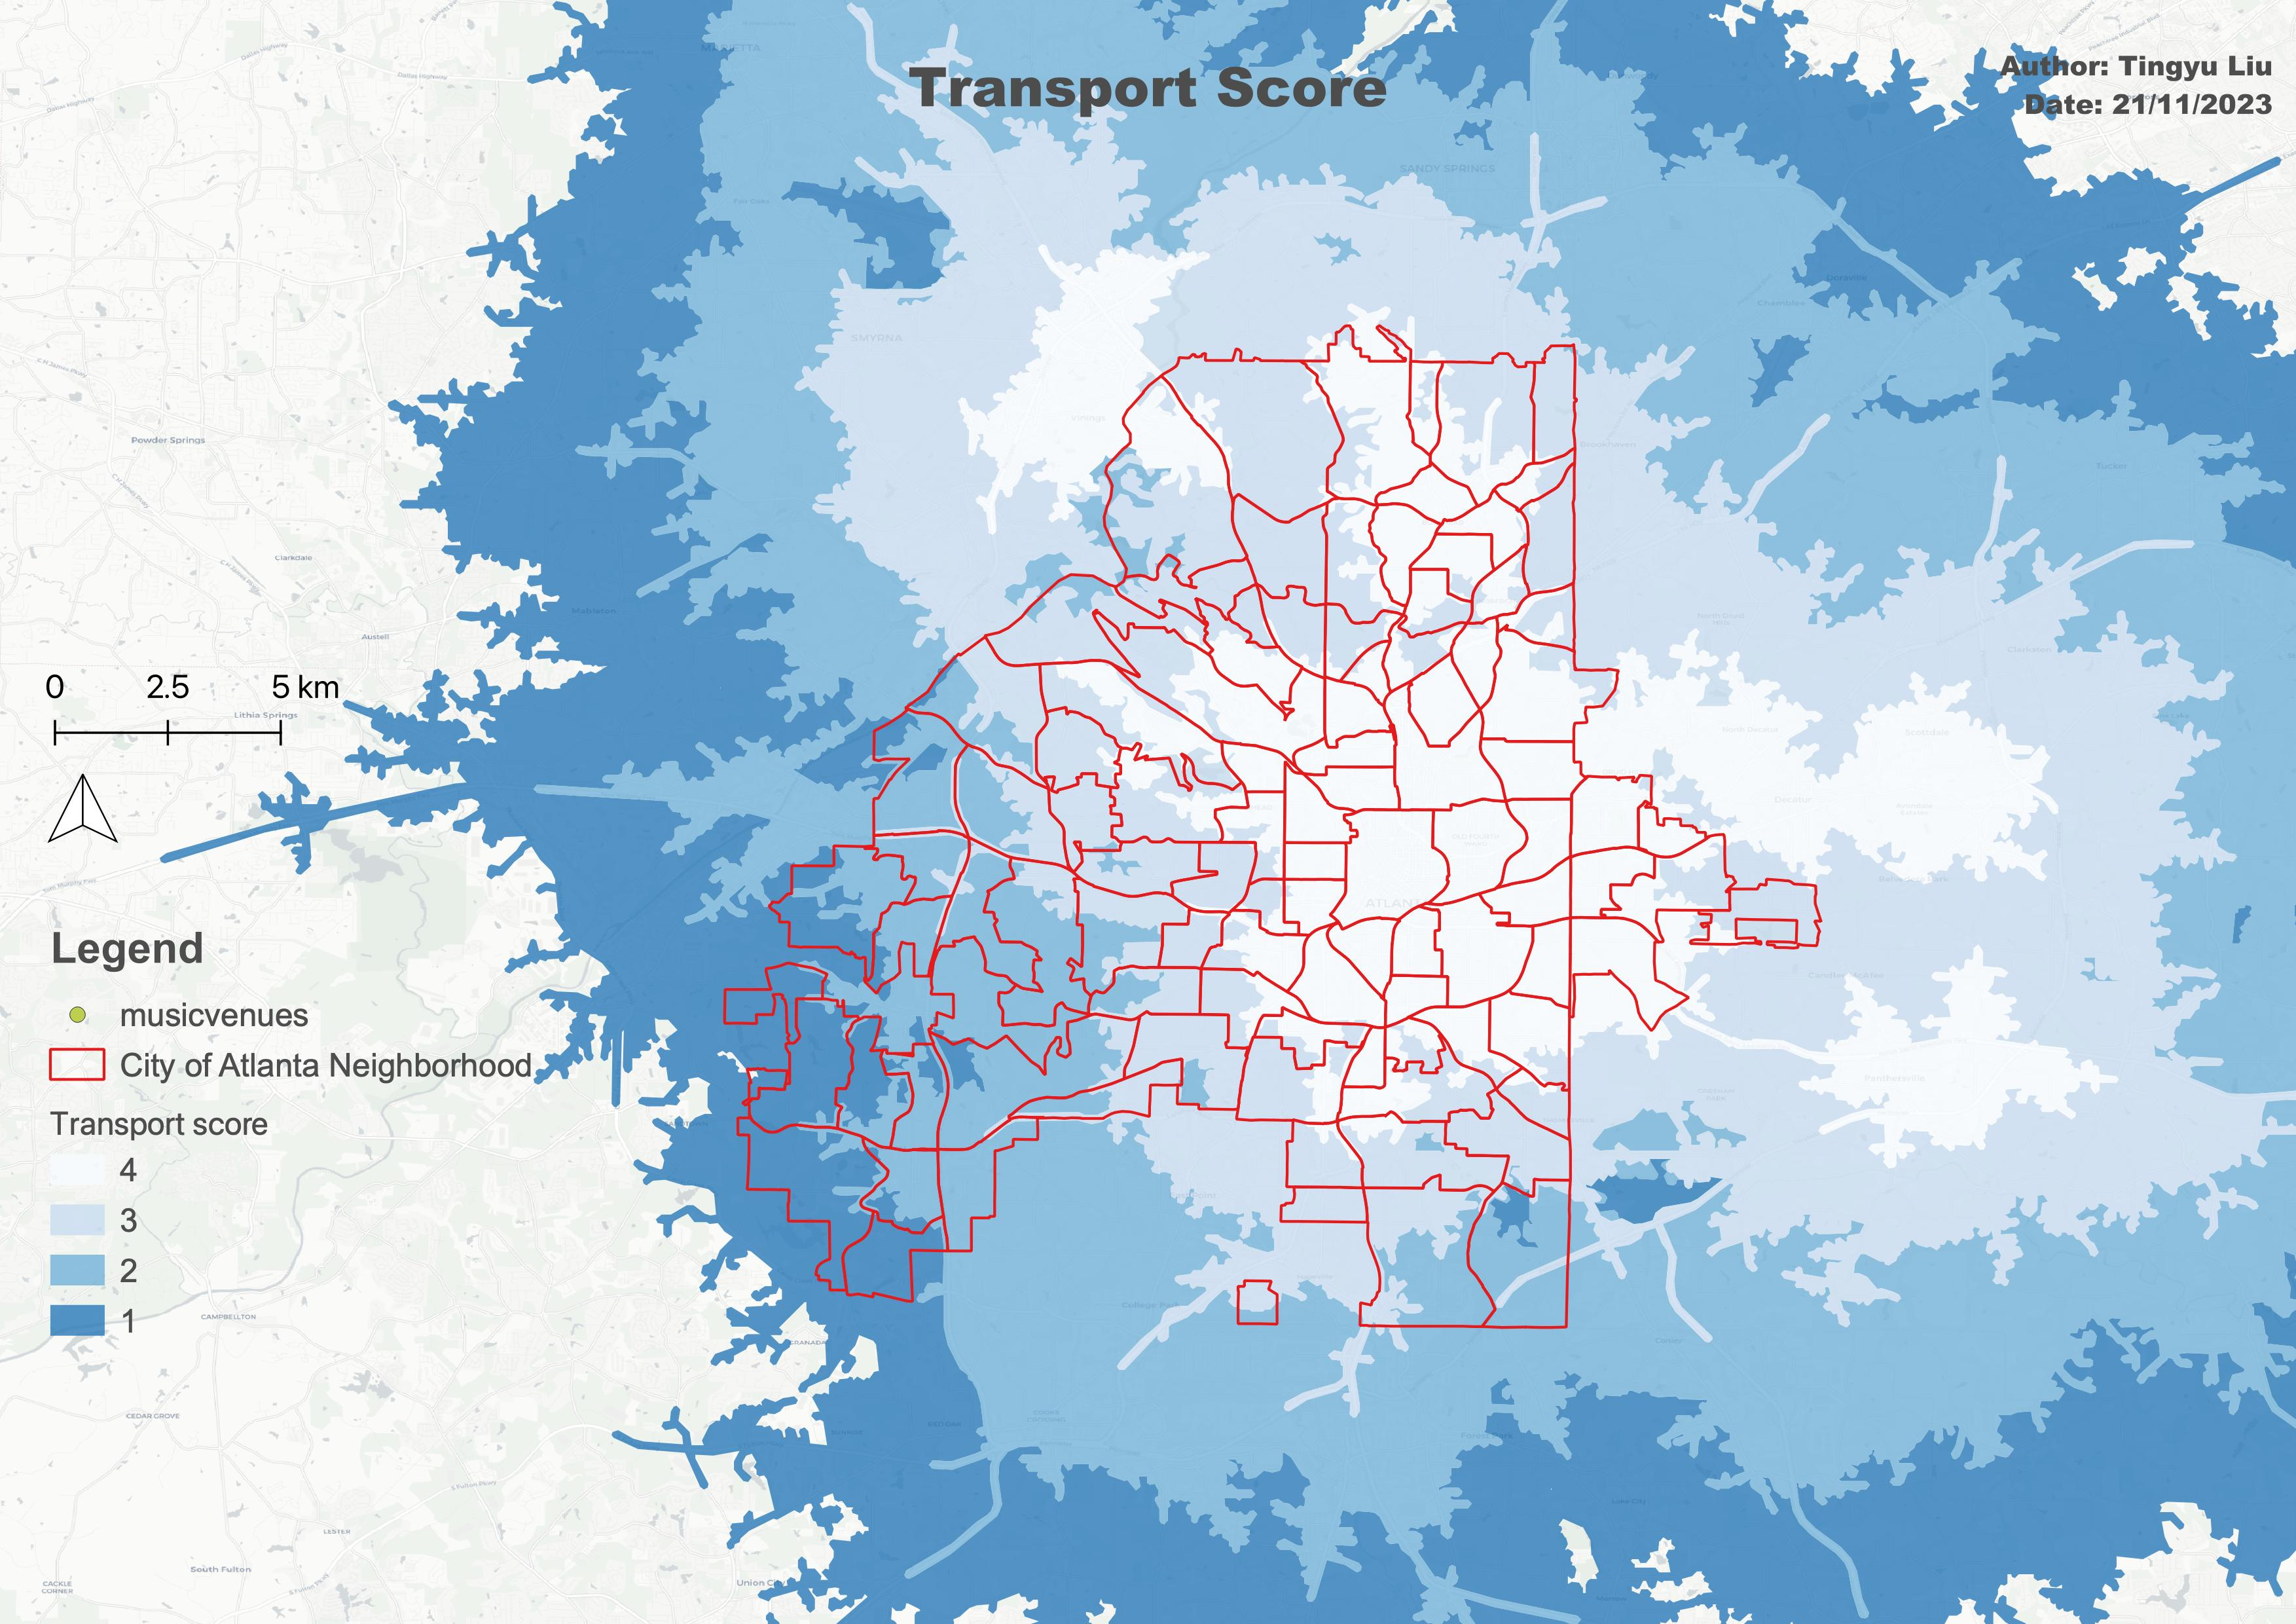
\includegraphics[width=0.48\textwidth]{map2/3_service score.jpg}%
        \label{fig:a}%
        }%
    \hfill%
    \subfloat{%
        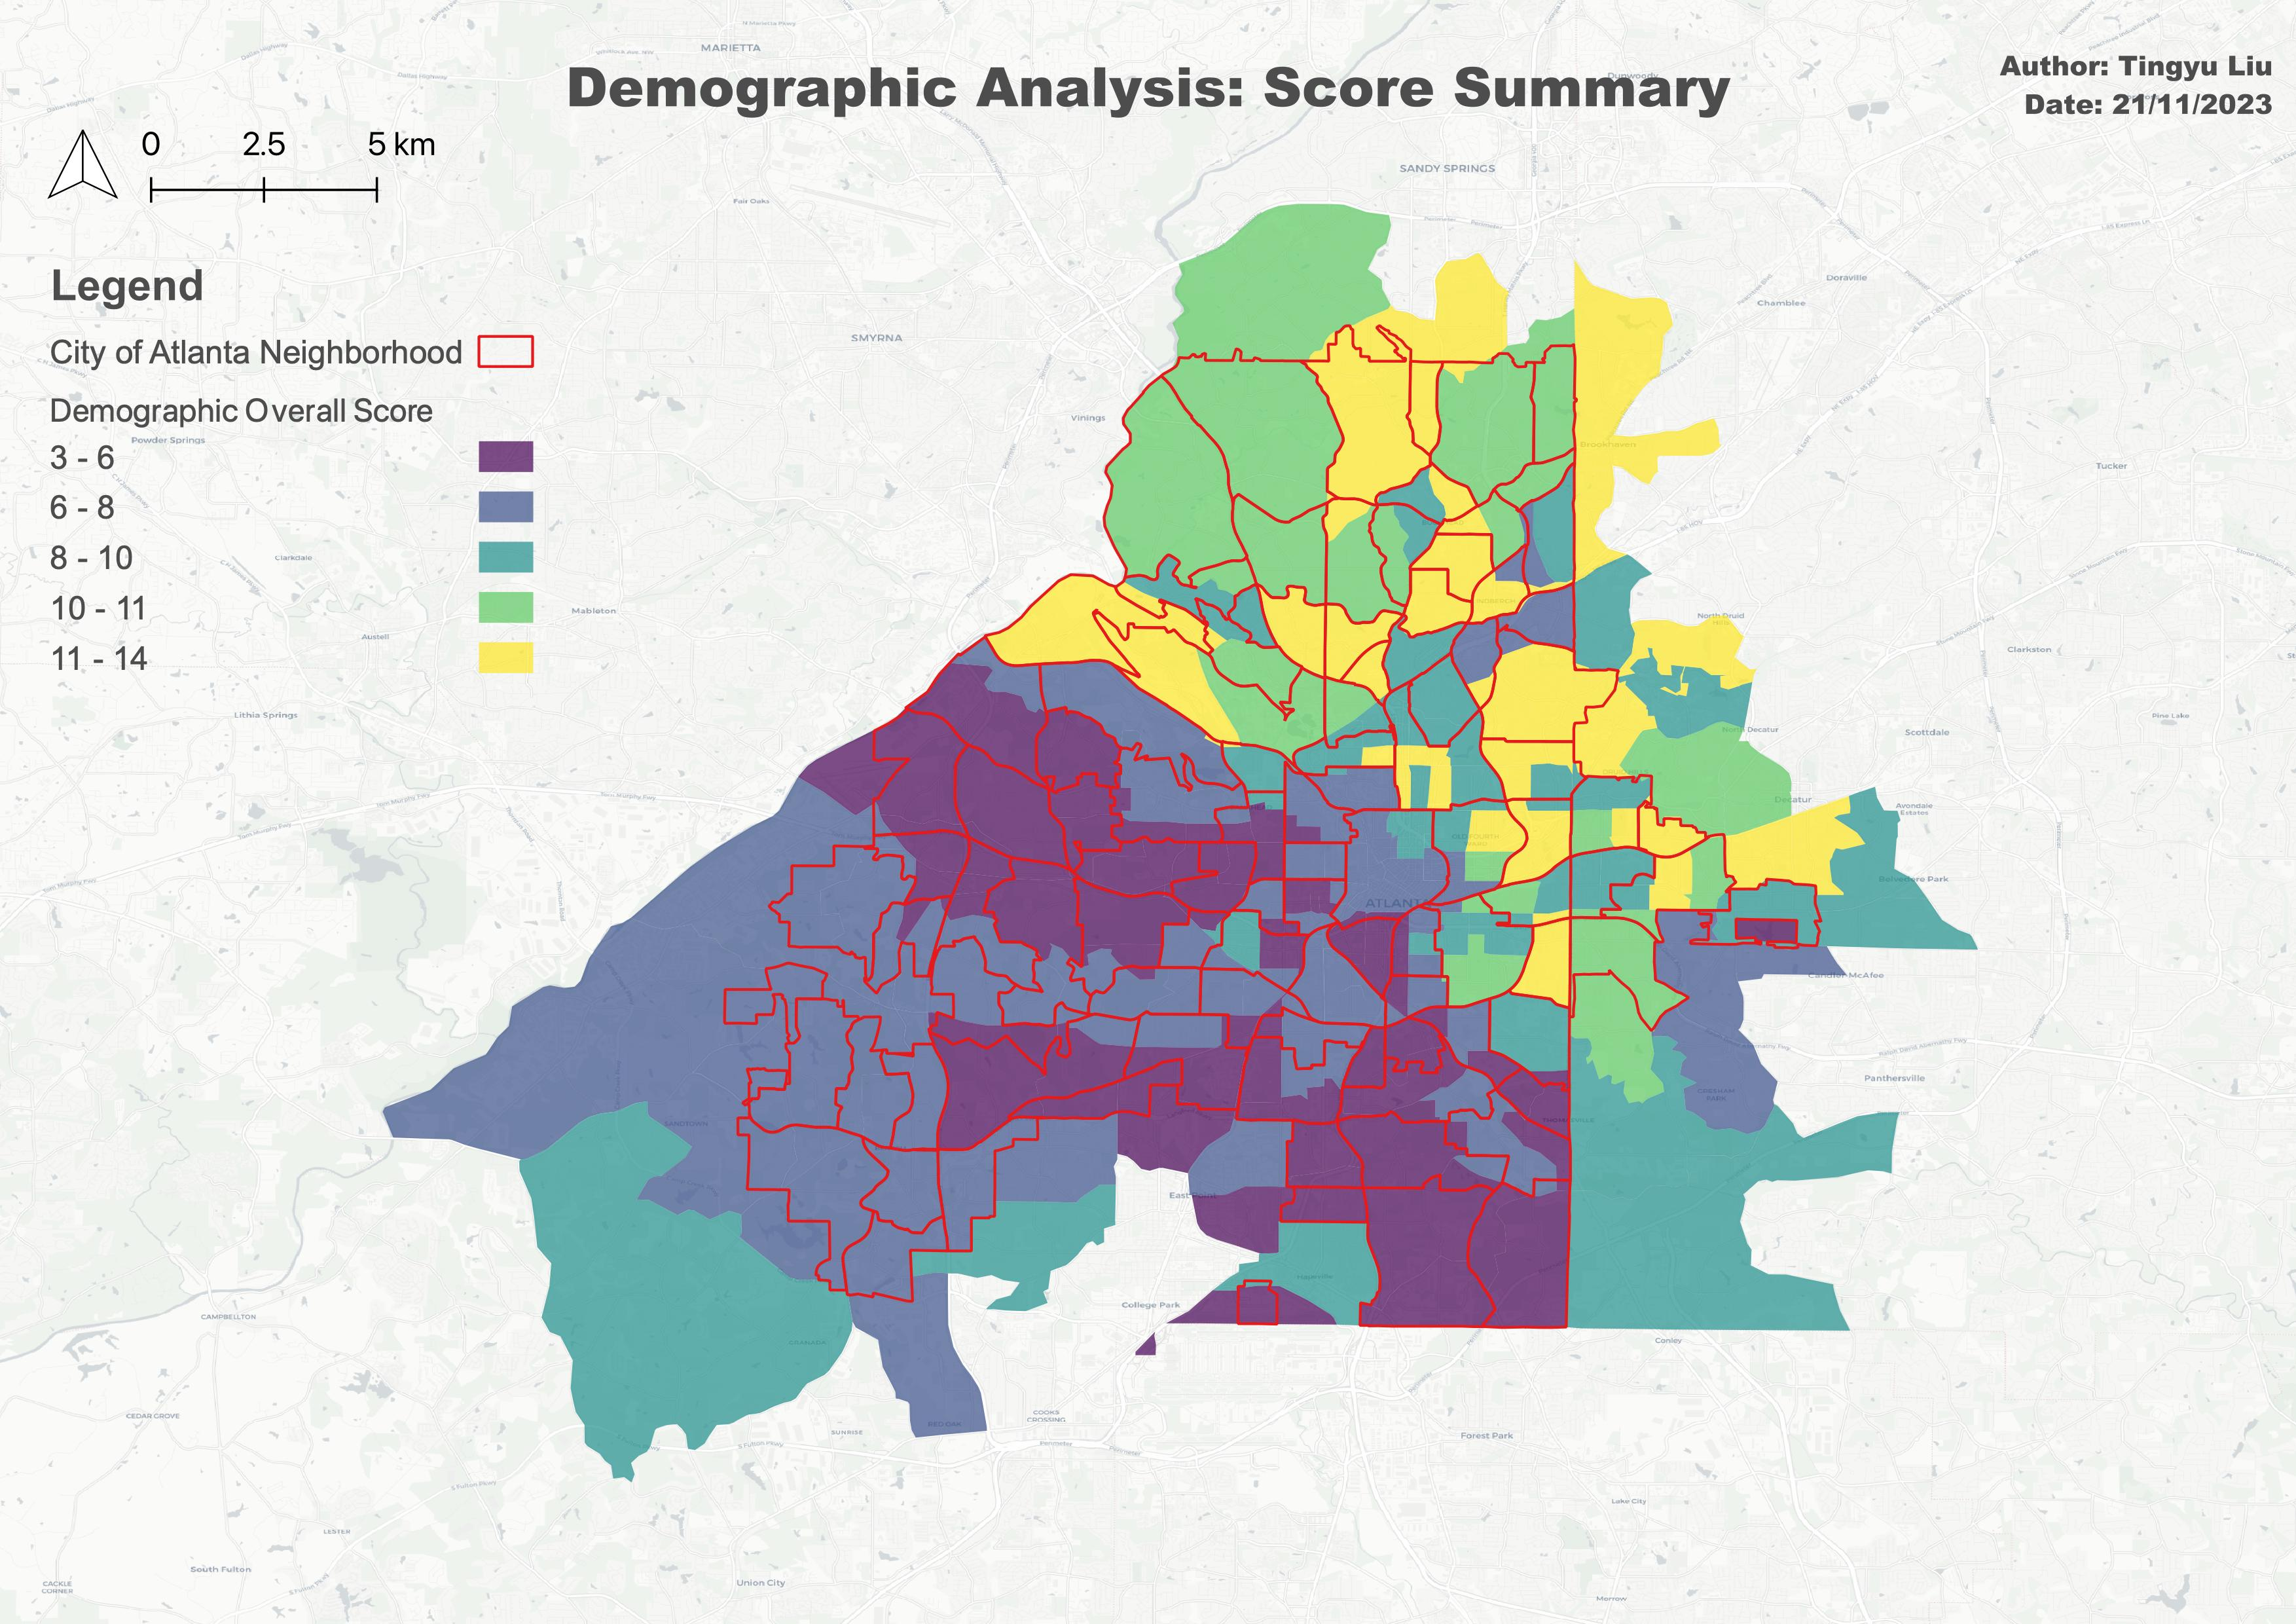
\includegraphics[width=0.48\textwidth]{map2/3_demographic summary.jpg}%
        \label{fig:b}%
        }%
    \caption{all the data}
\end{figure}

\begin{center}
\centering
Figure 10: Transport Analysis: Service Area Score \& Figure 11: Demographic Analysis: Total Demographic Score
\end{center}

\newpage

\textbf{Factor Integration}

Upon the integration of transport and demographic scores, the neighborhoods that emerge with the highest scores (16 out of a possible 18) are Midtown, Inman Park, East Atlanta, Peachtree Heights West, and Buckhead Forest. These neighborhoods exhibit advantageous conditions for the establishment of a metal music venue business, as evidenced by their accessibility, demographic composition, and urban planning factors. Through the quantification and amalgamation of these factors, the study identifies these neighborhoods as the most propitious locations for music venue business.

\begin{figure}[H]
\begin{center}
\centering
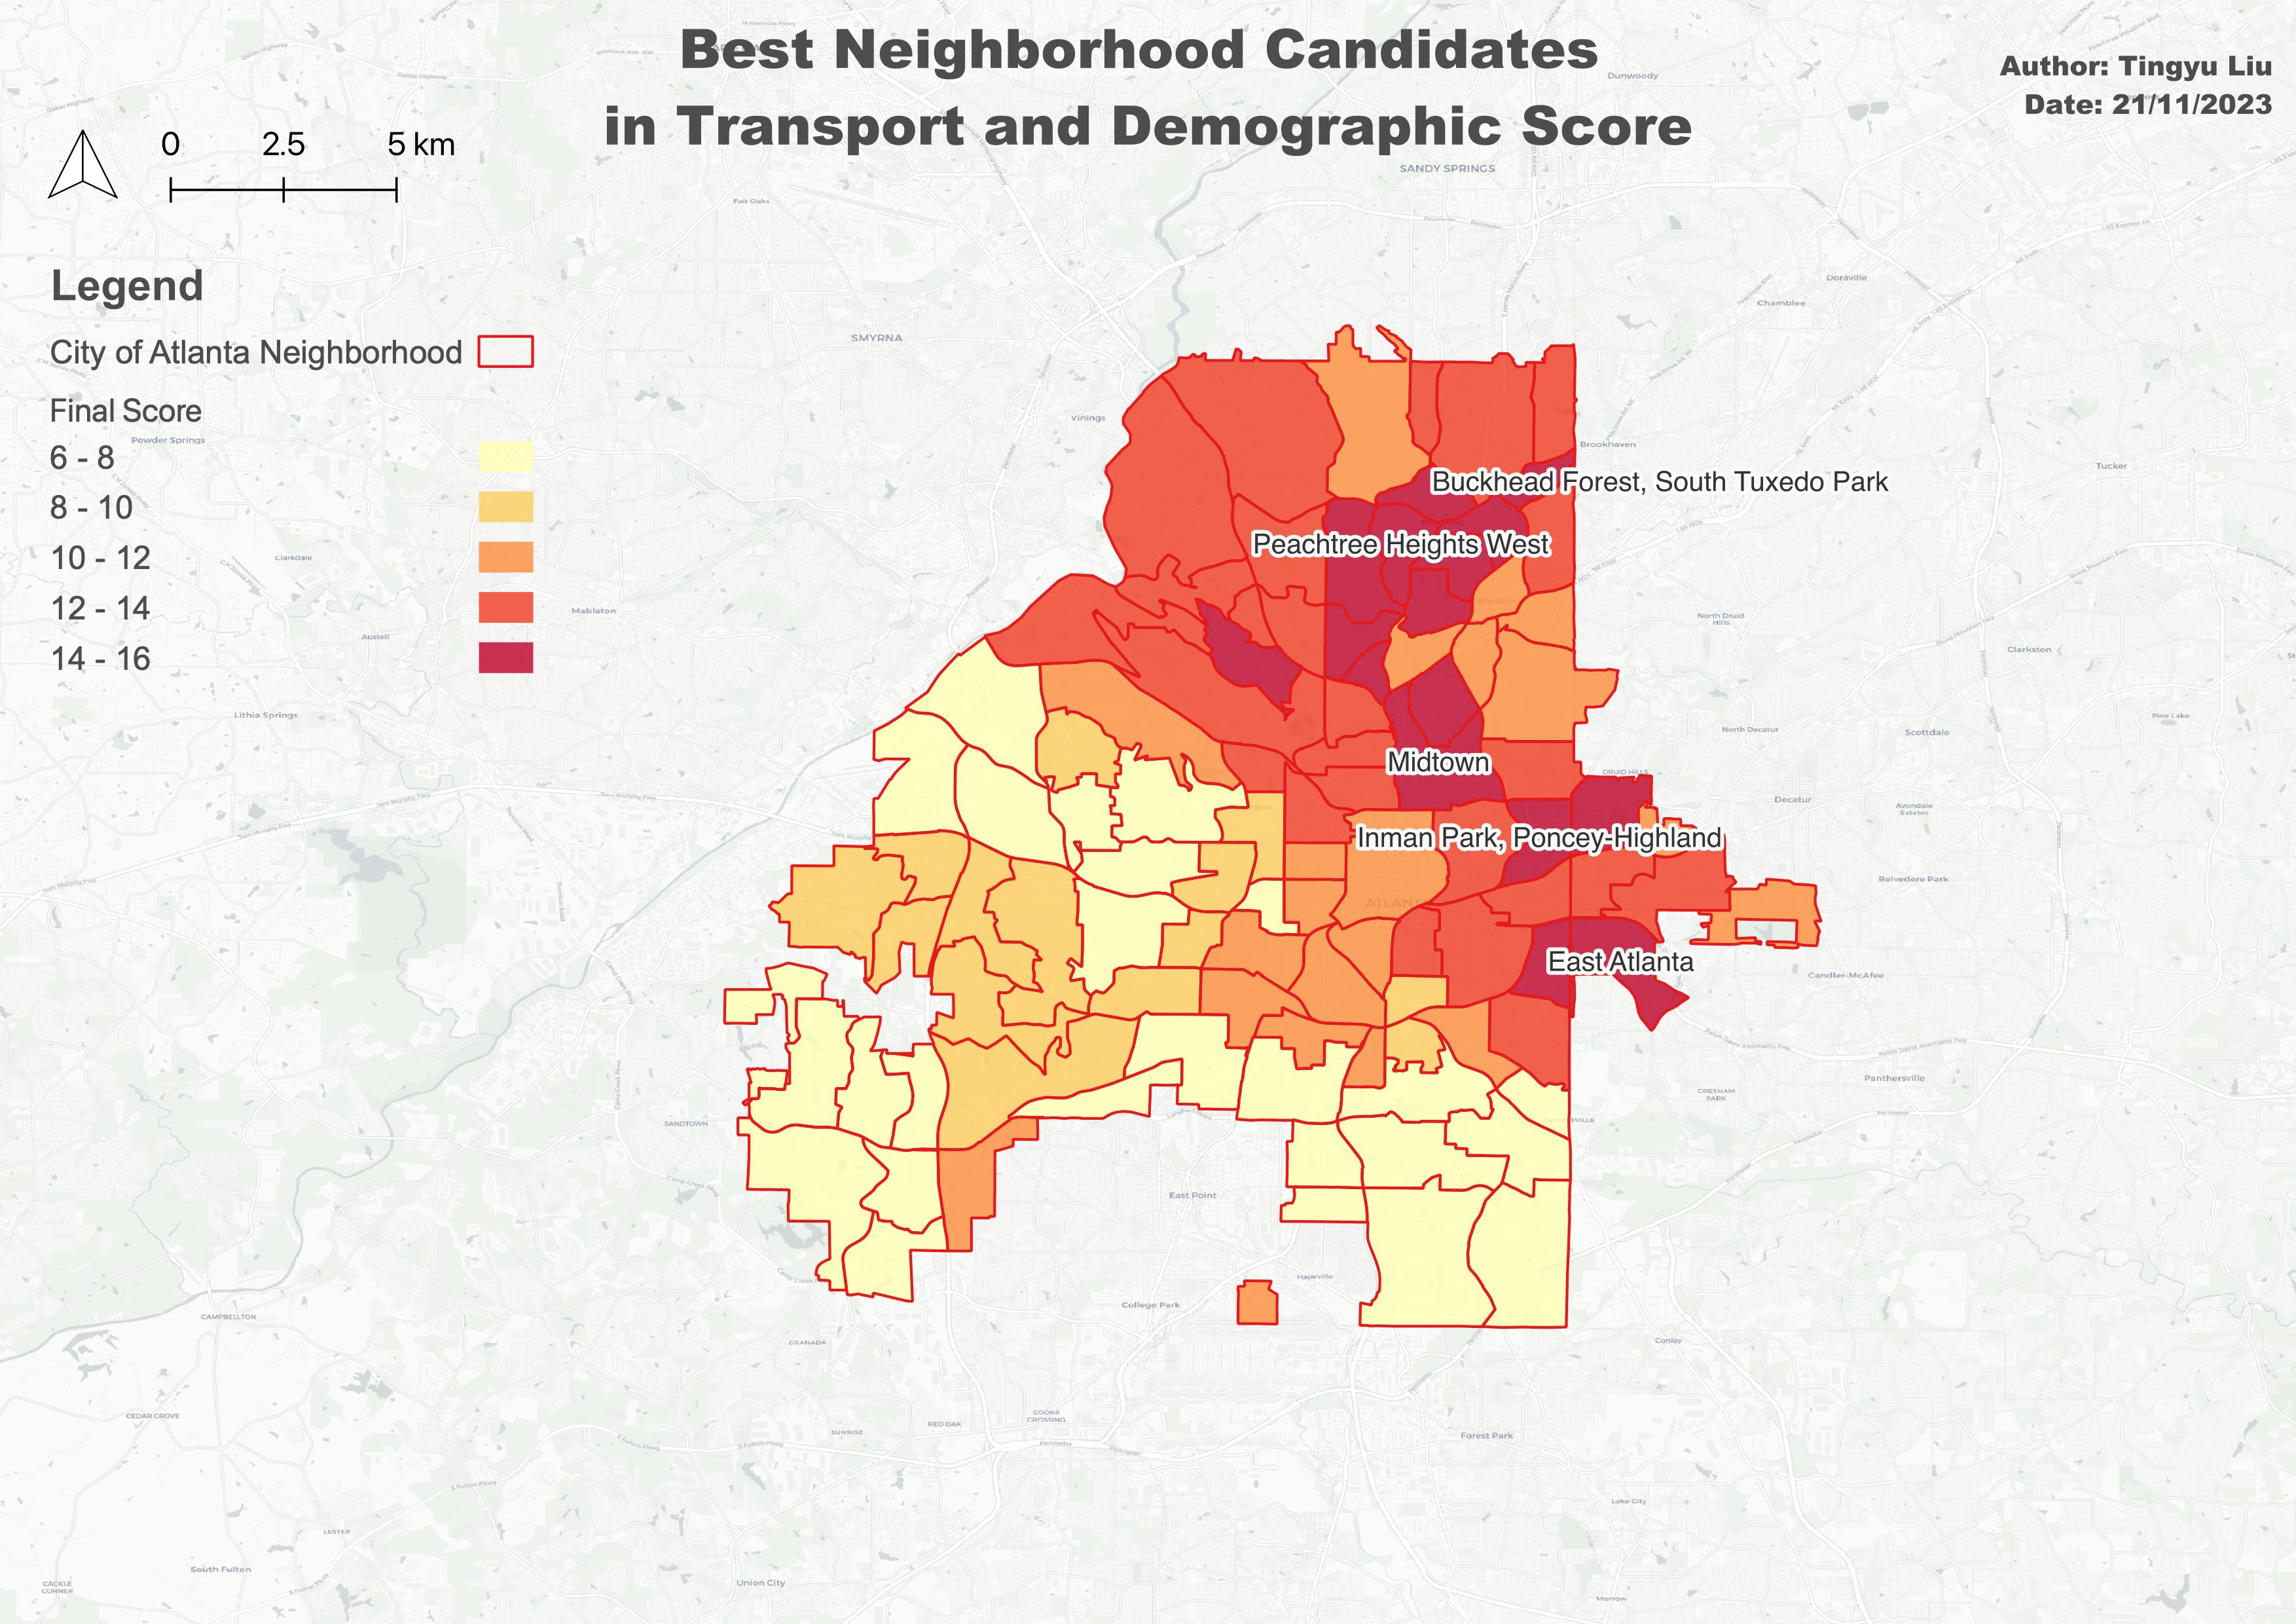
\includegraphics[width=1\textwidth]{map2/4_transport and demographic.jpg}
\caption{Figure 1: Different levels of urban development intensity}
\label{fig:figure1}
\end{center}
\end{figure}


\begin{center}
\centering
Figure 12: Final Score for Neighborhoods
\end{center}

\newpage
\textbf{Restriction Analysis}

The Midtown, Inman Park, and Buckhead Forest neighborhoods outperform others in terms of zoning and LCI restrictions. This is due to their higher proportion of commercial and mixed-landuse areas, as well as their larger overlay area with LCI. These factors indicate a better business atmosphere, greater popularity walkability, and stronger economic drive.

\begin{figure}[H]
\begin{center}
\centering
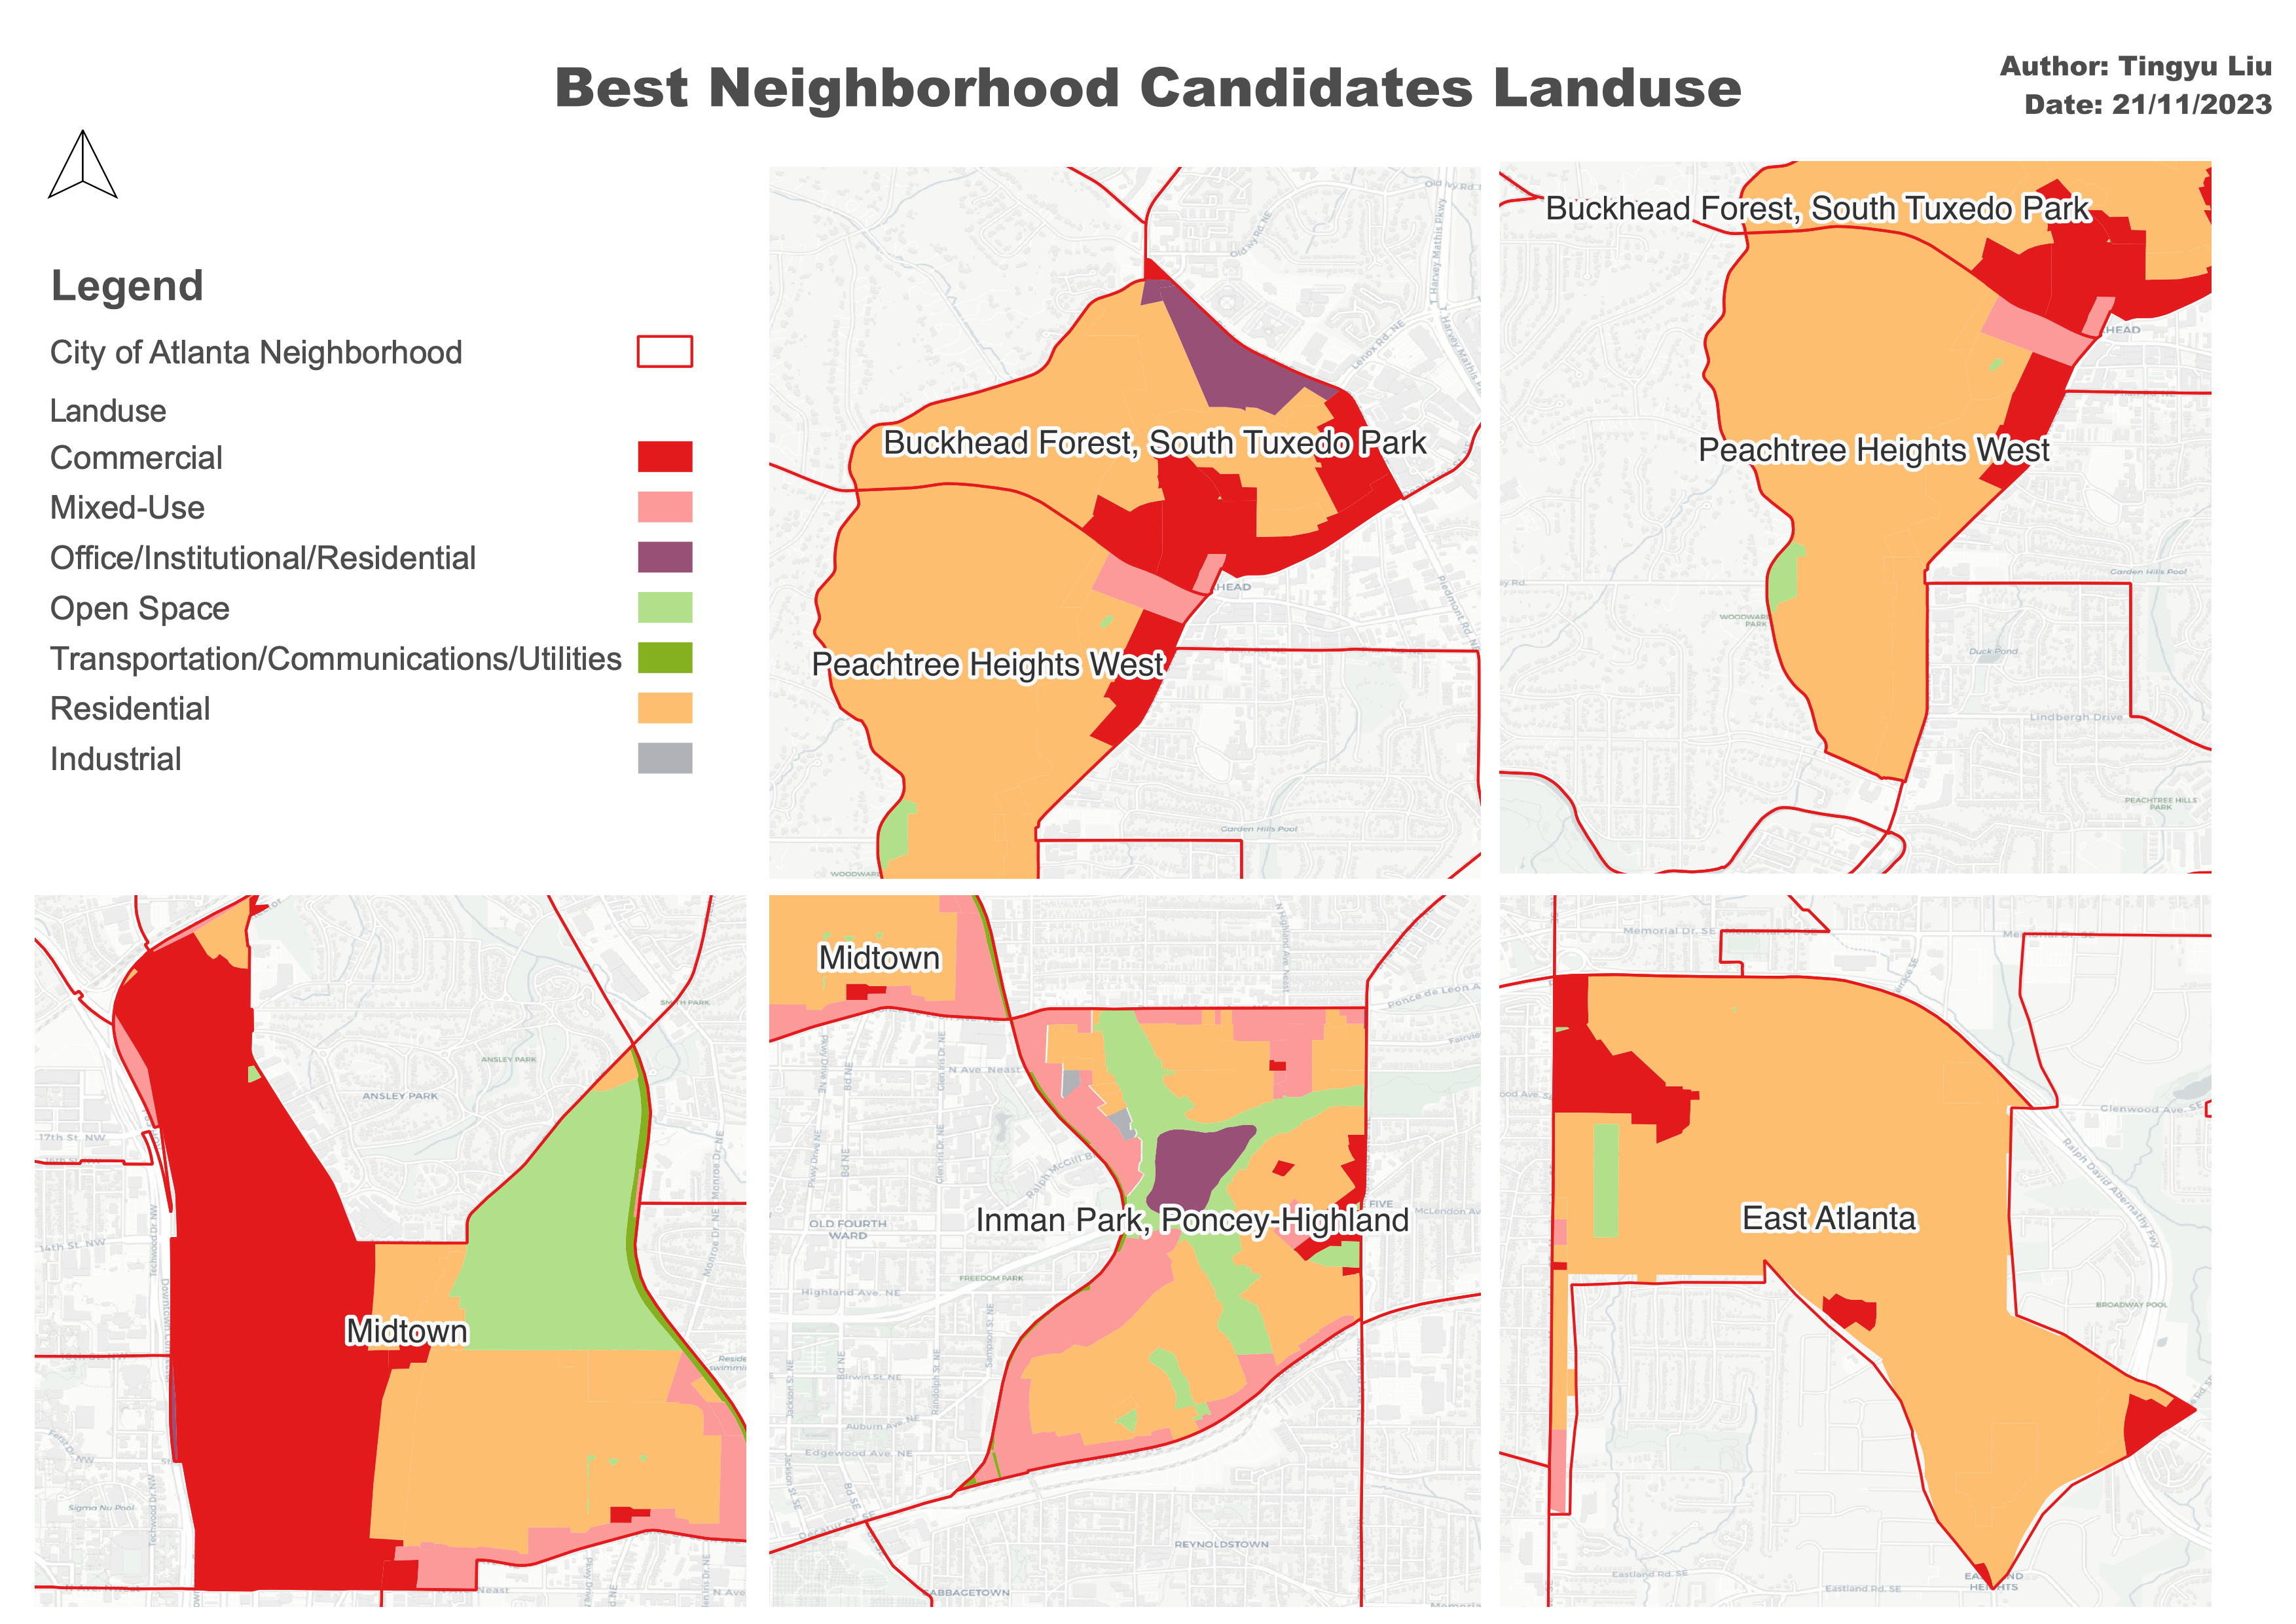
\includegraphics[width=0.7\textwidth]{map2/layout5- zoing restriction.png}
\caption{Figure 1: Different levels of urban development intensity}
\label{fig:figure1}
\end{center}
\end{figure}

\begin{figure}[H]
\begin{center}
\centering
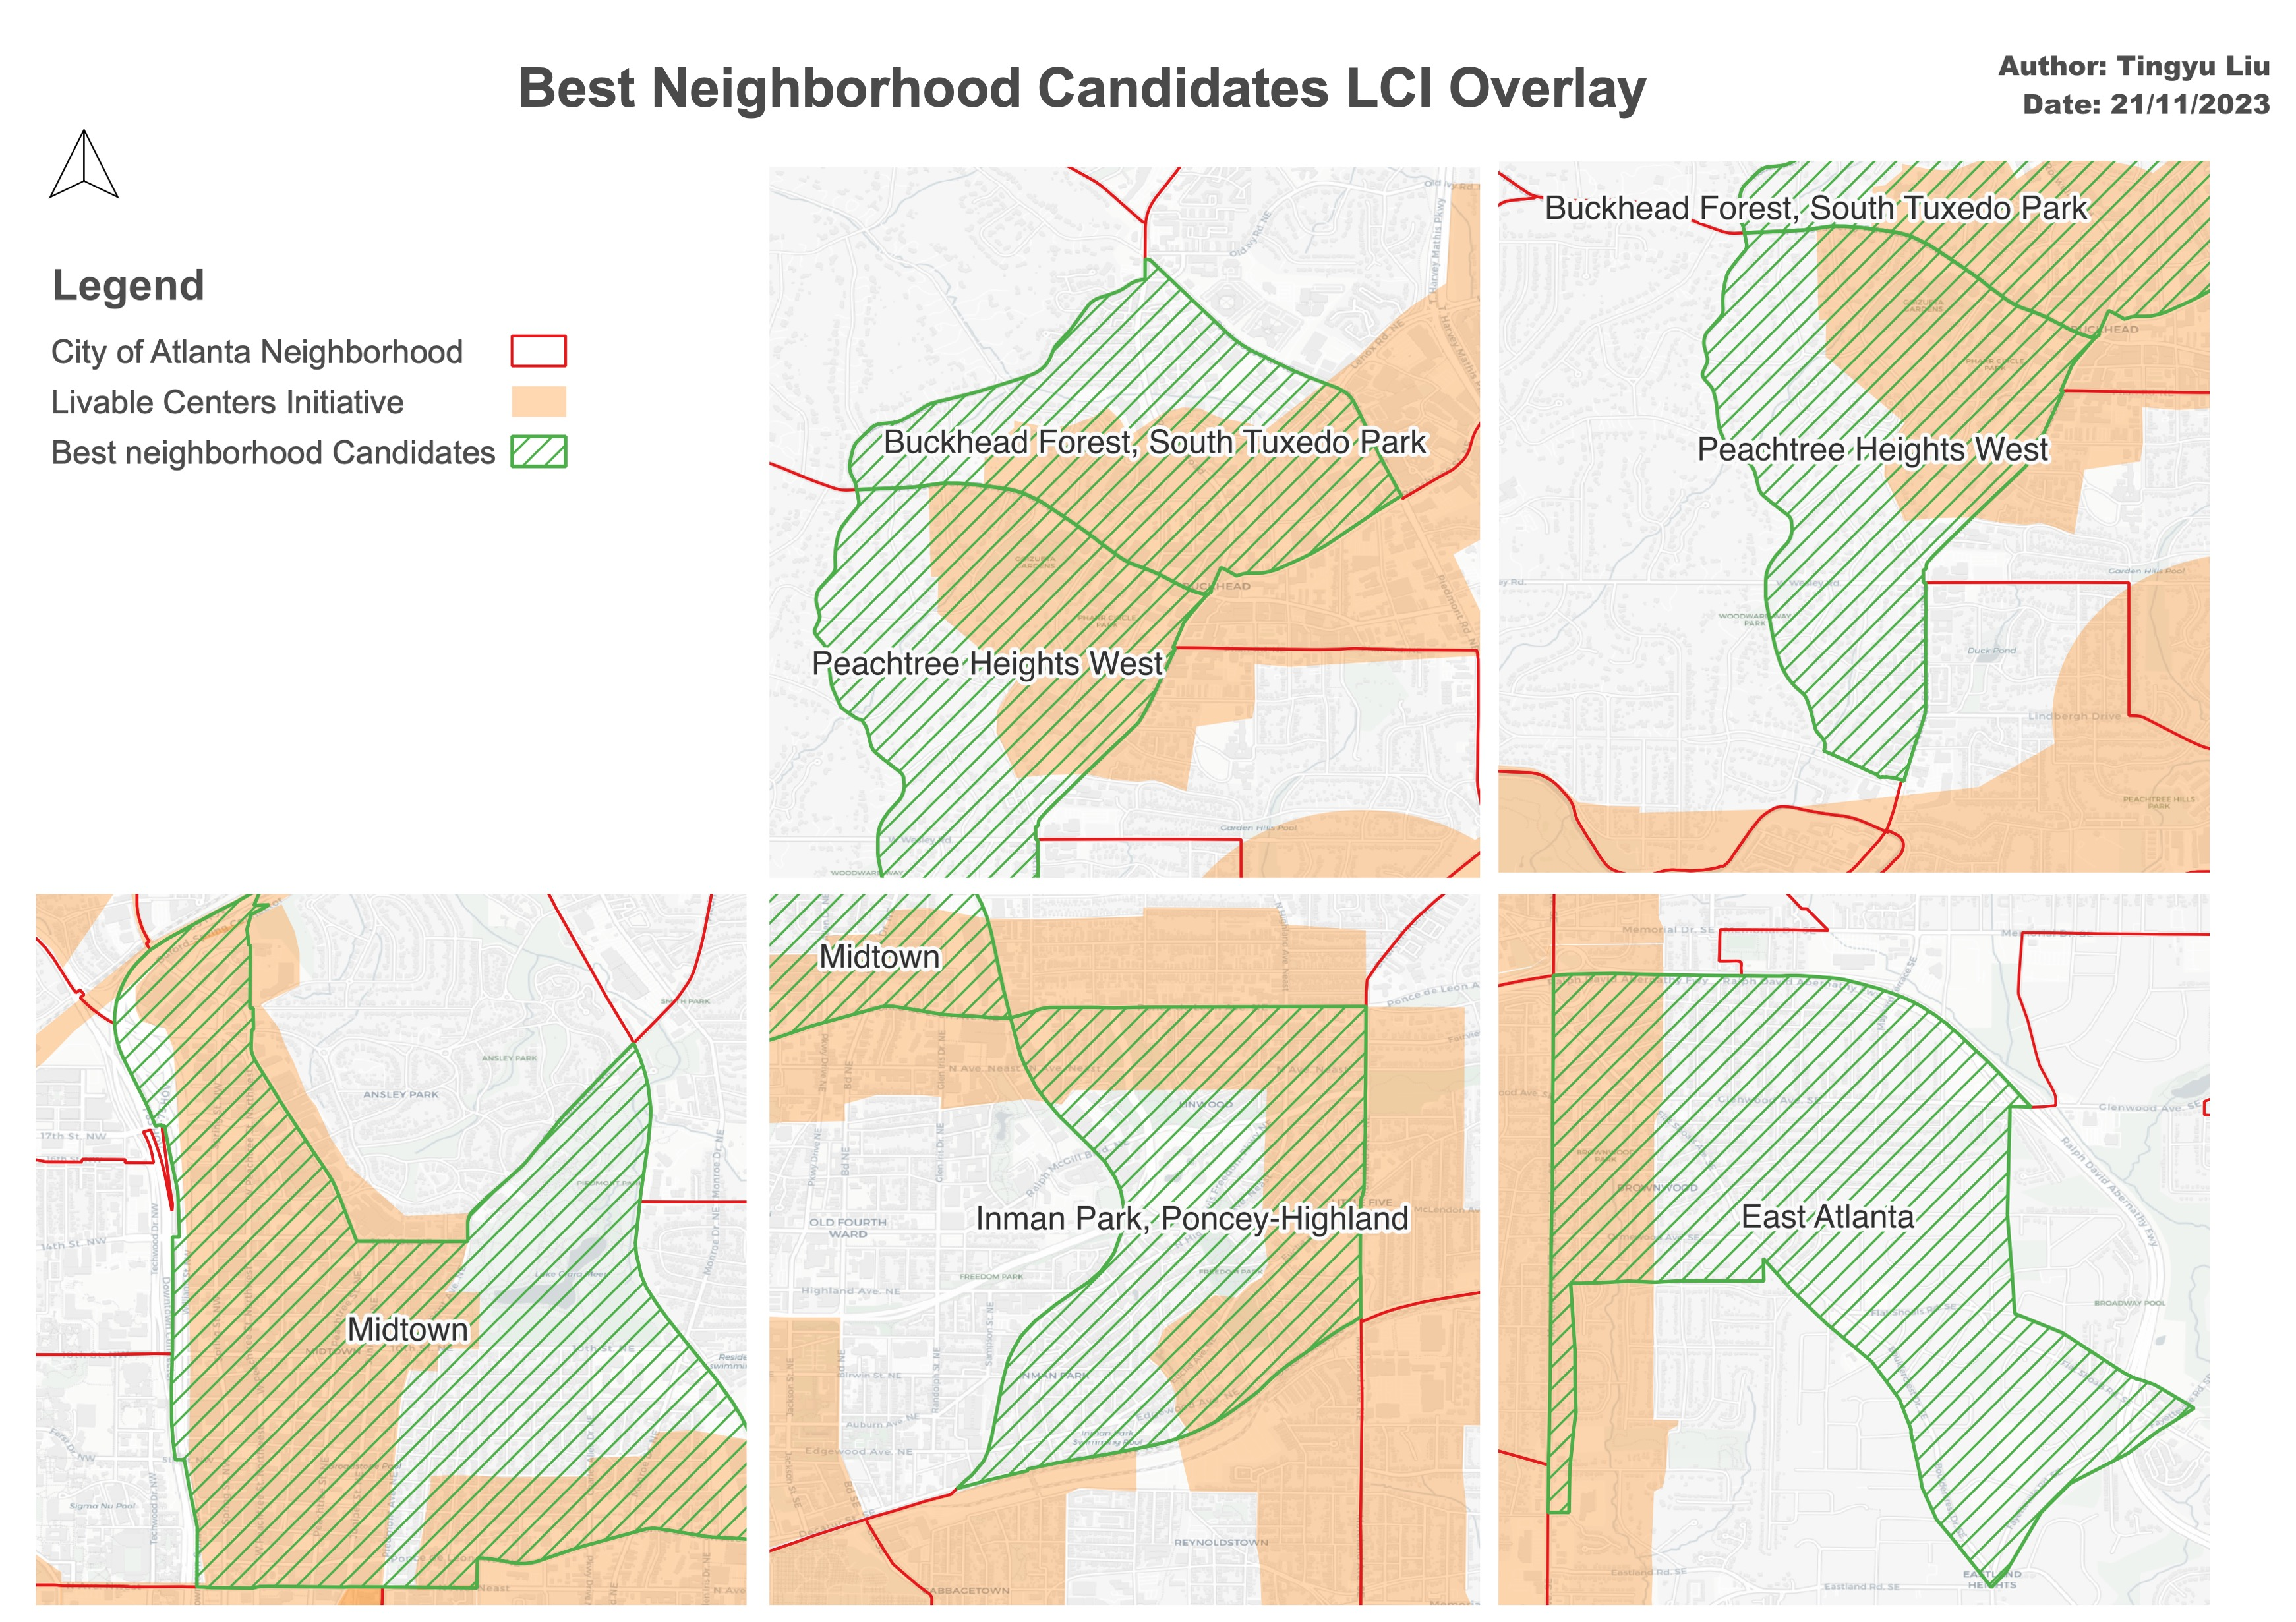
\includegraphics[width=0.6\textwidth]{map2/5_LCI.jpg}
\caption{Figure 1: Different levels of urban development intensity}
\label{fig:figure1}
\end{center}
\end{figure}

The figure illustrate the distribution of parking lot amenities within and in the vicinity of each potential neighborhood. 

Taking into account the availability of parking lots, Midtown and Inman Park emerge as the most viable options. This conclusion is drawn based on the current distribution and accessibility of parking facilities in these neighborhoods.

\begin{figure}[H]
\begin{center}
\centering
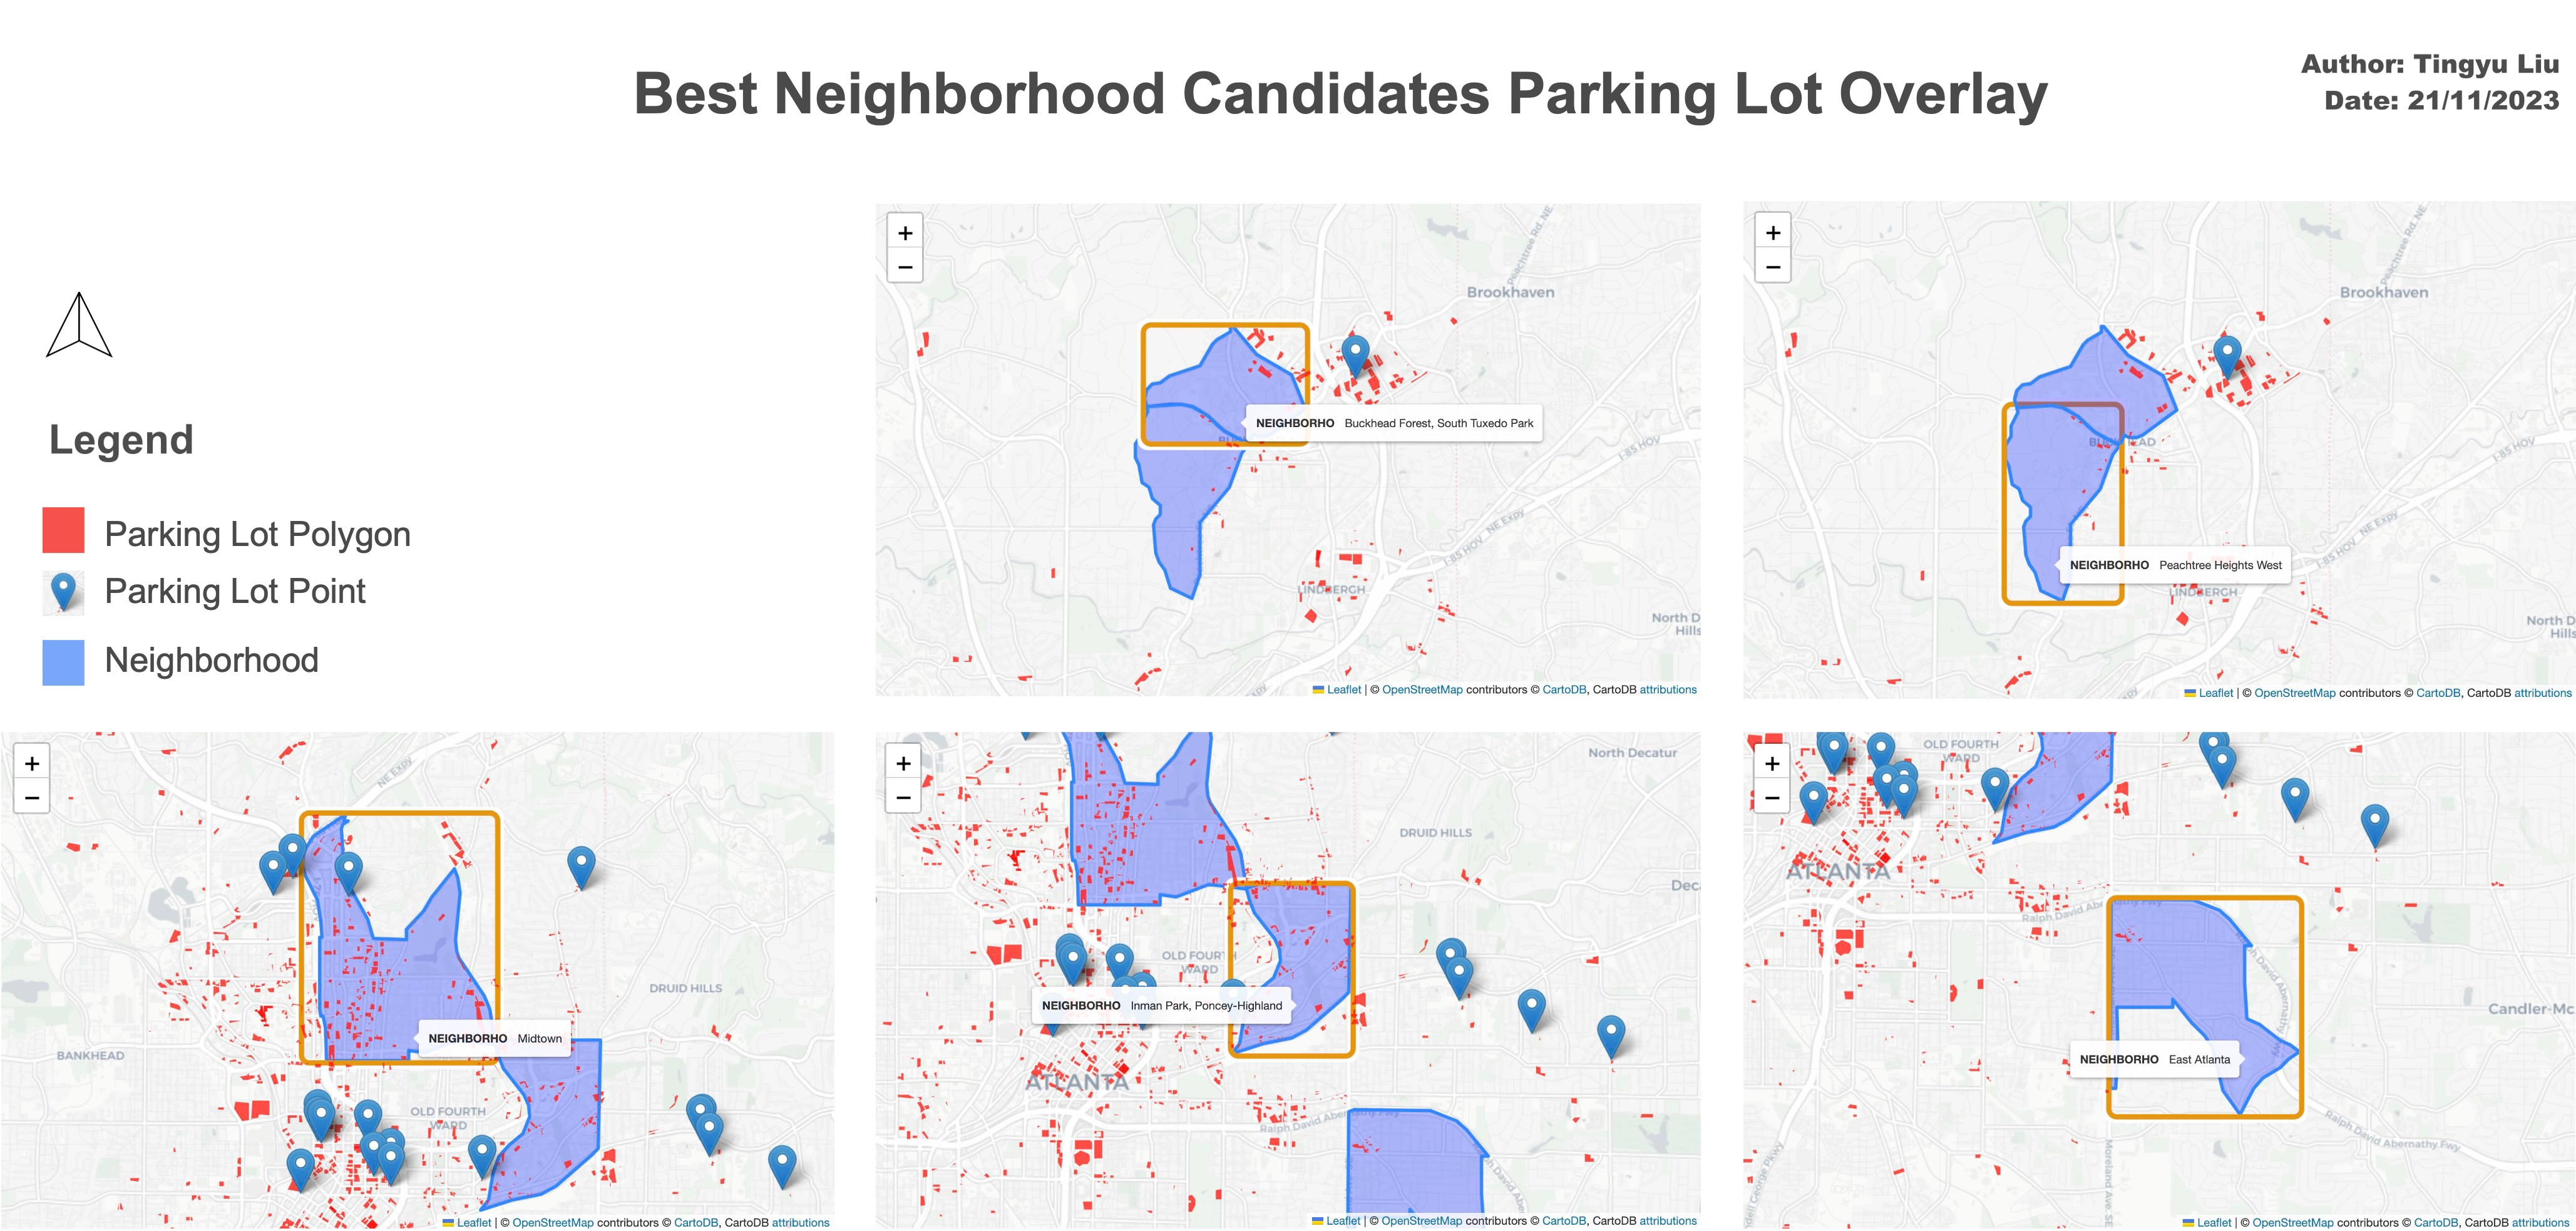
\includegraphics[width=1\textwidth]{map2/5_parking.jpg}
\caption{Figure 1: Different levels of urban development intensity}
\label{fig:figure1}
\end{center}
\end{figure}

\subsection{Conclusion}
Upon quantifying both transport and demographic factors, and imposing transport and urban planning factors as constraints, the study concludes that Midtown and Inman Park emerge as the most favorable locations for establishing a metal music venue business.

Midtown, with its well-established music venue business, presents a competitive landscape. It is likely to resonate with the metal music enthusiasts due to its familiarity. However, it is pertinent to note that this venture in Midtown could be characterized as high-risk, high-reward.

On the other hand, Inman Park, with fewer existing music venues, exhibits a higher potential for this business, given the suitable conditions it offers. The proposed location for the music venue is Edgewood Avenue, renowned for its restaurant street. However, it is important to consider that the real estate prices in this area are comparatively higher. This factor could influence the overall feasibility of the venture.

\subsection{Discussion}

This study assesses the spatial distribution and service area of existing music venues in Atlanta. It identifies neighborhoods with high potential for establishing metal music venues, considering transportation, demographic, and urban planning factors. The study utilizes two procedures: quantitative matrices ranking and restriction analysis, as spatial and mathematical models.


\textbf{Merits and Long-term Effects}

This study stands out due to its innovative and interdisciplinary approach in transport, GIS, urban planning, and sociology. It integrates concepts from different fields, creating a comprehensive model for location analysis. Furthermore, the research is vertical in nature, delving deep into the subject matter to provide nuanced insights. Also, this study combines city-level location analysis with business-level user profiling. This combination allows for a more holistic understanding of the factors influencing the success of a music venue business.

The long-term effects of this project include promoting a vibrant music scene in Atlanta and providing valuable insights for businesses looking to establish a metal music venue in the city.

\textbf{Uncertainty and Error}

The potential for uncertainty and error in this project primarily stems from the accuracy of the data sources and the assumptions inherent in the spatial and mathematical models.

\textbf{Data Source Uncertainty and Error}

As discussed in the data accuracy section, the data sources, particularly the point of interest data for music venues from Yelp, contain inherent uncertainties and errors. It is worth noting that certain establishments, such as bars and restaurants that host live metal music shows, may not be categorized as music venues and are therefore excluded from this project. For instance, \textit{Boggs Social \& Supply}, despite hosting significant metal music events, is categorized as a bar, food truck, or breakfast point of interest, and is not included in the music venue data.

\textbf{Assumptions in the Spatial and Mathematical Model}

While this study integrates various fields and employs a comprehensive model, the complexity of real-life location analysis extends beyond the scope of this research. For example, the process of opening a music venue is influenced by factors such as the investor’s social network (Tai, 2014), which are not accounted for in the current model.


\textbf{Further Work}

The integration of machine learning methodologies could potentially enhance the sophistication of the analyses and predictions, thereby revealing patterns and relationships that may not be immediately apparent in the current study. For instance, if data pertaining to metal music venues, transport, and demographics is collected on a national scale and subsequently subjected to rigorous cleaning processes, the application of Principal Component Analysis (PCA) could augment interpretability while simultaneously preserving the maximum amount of information. This could facilitate the identification of features that render a neighborhood suitable for music venues.

Future research could employ Natural Language Processing (NLP) to extract insights from metalheads and venue owners, aiding in identifying locations that optimize social, cultural, and business capital. Additionally, Latent Dirichlet Allocation (LDA) topic modeling in Location-Based Social Networks (LSBN) could reveal meaningful topics and functional regions based on Point of Interest (POI) co-occurrence patterns, enhancing our understanding of metal music enthusiasts’ activities and music venue analysis (Gao et al., 2017).




\newpage

\section{Reference}

{[}1{]} Florida, R., Jackson, S. (2010). Sonic City: The Evolving Economic Geography of the Music Industry. Journal of Planning Education and Research, 29(3), 310-321. https://doi.org/10.1177/0739456X09354453

{[}2{]} Castro, G. (2017, October 26). Mass Destruction Metal Fest Set to Put the Southeast on the Metal Map - Immersive Atlanta. Immersive Atlanta | Atlanta Music, Arts and Culture. https://immersiveatlanta.com/mass-destruction-metal-fest-set-to-put-the-southeast-on-the-metal-map/

{[}3{]} 2021 CDP - Atlanta Department of City Planning. (n.d.). Atlanta Department of City Planning. Retrieved December 10, 2023, from https://www.atlcitydesign.com/2021-cdp)

{[}4{]} Whiting, S. (2021). The Value of Small Live Music Venues: Alternative Forms of Capital and Niche Spaces of Cultural Production. Cultural Sociology, 15(4), 558-578. https://doi.org/10.1177/17499755211021307

{[}5{]} \textit{Carah, N., Regan, S., Goold, L., Rangiah, L., Miller, P., Ferris, J. (2021). Original live music venues in hyper-commercialised nightlife precincts: exploring how venue owners and managers navigate cultural, commercial and regulatory forces. International Journal of Cultural Policy, 27(5), 621-635. https://doi.org/10.1080/10286632.2020.1830979}

{[}6{]} Tai, Y. (2014). \textit{You Can't Always Get What You Want: Gatekeeping and Social Capital in the Live-Music Scenes of Atlanta and Taipei} (Order No. 3639931). Available from ProQuest Dissertations \& Theses A\&I; ProQuest Dissertations \& Theses Global. (1614473153). https://www.proquest.com/dissertations-theses/you-cant-always-get-what-want-gatekeeping-social/docview/1614473153/se-2

{[}7{]} Walser, R. (1993). Running with the devil: Power, gender, and madness in heavy metal music. Wesleyan University Press.

{[}8{]} Yelp Business Search API. (n.d.). Yelp. Retrieved from \textit{https://www.yelp.com/developers/documentation/v3/business\_search}

{[}9{]} Census Bureau API. (n.d.). U.S. Census Bureau. Retrieved from https://www.census.gov/data/developers/data-sets.html

{[}10{]} American Community Survey 5-year estimates for 2019. (n.d.). U.S. Census Bureau. Retrieved from https://www.census.gov/data/developers/data-sets/acs-5year.html

{[}11{]} Boeing, G. 2017. OSMnx: New Methods for Acquiring, Constructing, Analyzing, and Visualizing Complex Street Networks. Computers, Environment and Urban Systems 65, 126-139.

{[}12{]} Fulton County, Georgia. Open Data. Retrieved November 23, 2023, from https://gisdata.fultoncountyga.gov/

{[}13{]} Accuracy. (2020, December 28). OpenStreetMap Wiki, . Retrieved 20:12, December 10, 2023 from https://wiki.openstreetmap.org/w/index.php?title=Accuracy\&oldid=2079309.

{[}14{]} Shukla, A. (2022). The Social Psychology Of Heavy Metal \& Rock Music: Research On Metalheads. \textit{Cognition Today}. Retrieved September 19, 2022.

{[}15{]} Gutiérrez, J., & García-Palomares, J. C. (2008). Distance-Measure Impacts on the Calculation of Transport Service Areas Using GIS. Environment and Planning B: Planning and Design, 35(3), 480-503. https://doi.org/10.1068/b33043

{[}16{]}Gao, S., Janowicz, K., & Couclelis, H. (2017). Extracting urban functional regions from points of interest and human activities on location‐based social networks. Transactions in GIS, 21(3), 446-467.













    % Add a bibliography block to the postdoc
    
    
    
\end{document}
